\documentclass[12pt]{article}
\usepackage[T2A,T1]{fontenc}
\usepackage[bulgarian]{babel}
\usepackage[utf8]{inputenc}
\usepackage[margin=1in]{geometry}% Change the margins here if you wish.
\usepackage{amsmath,amsthm,amssymb}
\usepackage{subcaption}
\usepackage{graphicx}
\usepackage{float}
\usepackage{titling}
\usepackage[colorlinks=true,linkcolor=blue,citecolor=red,unicode]{hyperref}
\usepackage{cancel}
\usepackage{tocstyle} % Table of contents formatting
\usepackage{epsfig} % EPS file format in figures
\usepackage{booktabs} % For better lines in tables

%%% --------------------- CONFIGURATION ---------------------

\setlength{\parindent}{0pt} % This is the set the indent length for new paragraphs, change if you want.
\setlength{\parskip}{10pt} % This sets the distance between paragraphs, which will be used anytime you have a blank line in your LaTeX code.

% Renames the subsection links in appendix to use the appendix name
% begin appendix autoref patch [\autoref subsections in appendix](https://tex.stackexchange.com/questions/149807/autoref-subsections-in-appendix)
\usepackage{etoolbox}
\makeatletter
\patchcmd{\hyper@makecurrent}{%
    \ifx\Hy@param\Hy@chapterstring
        \let\Hy@param\Hy@chapapp
    \fi
}{%
    \iftoggle{inappendix}{%true-branch
        % list the names of all sectioning counters here
        \@checkappendixparam{chapter}%
        \@checkappendixparam{section}%
        \@checkappendixparam{subsection}%
        \@checkappendixparam{subsubsection}%
        \@checkappendixparam{paragraph}%
        \@checkappendixparam{subparagraph}%
    }{}%
}{}{\errmessage{failed to patch}}
\newcommand*{\@checkappendixparam}[1]{%
    \def\@checkappendixparamtmp{#1}%
    \ifx\Hy@param\@checkappendixparamtmp
        \let\Hy@param\Hy@appendixstring
    \fi
}
\makeatletter
\newtoggle{inappendix}
\togglefalse{inappendix}
\apptocmd{\appendix}{\toggletrue{inappendix}}{}{\errmessage{failed to patch}}
%\apptocmd{\subappendices}{\toggletrue{inappendix}}{}{\errmessage{failed to patch}}
% end appendix autoref patch

% Redefine subsection numbering
%\renewcommand\thesubsection{\roman{subsection})}
% Redefine the autoref names
\renewcommand{\equationautorefname}{Уравнение}
\renewcommand{\appendixautorefname}{Приложение}
\renewcommand{\figureautorefname}{Фиг.}
\renewcommand{\tableautorefname}{Таблица}
% Add section number to the equation numbering
\numberwithin{equation}{section}

% Commonly used macros

% Just v with arrow on top
\newcommand{\vel}{\vec{v}}
% Puts and underbrace under the first argument, equal sign and then the second argument below
\newcommand{\DefineAs}[2]{\underset{\overset{\shortparallel}{#2}}{\underbrace{#1}}}

%%% --------------------- DOCUMENT ---------------------

\begin{document}

\thispagestyle{empty} % Hide the page number for the first page
\begin{center}
    {\large
    \includegraphics[width=0.15\textwidth]{SU.png} \\
    СОФИЙСКИ УНИВЕРСИТЕТ ,,СВ. КЛИМЕНТ ОХРИДСКИ'' \\
    ФАКУЛТЕТ ПО МАТЕМАТИКА И ИНФОРМАТИКА\\
    Катедра ,,Числени методи и алгоритми''
    }
    
    \hrulefill

    \vspace{5em}
    {\Huge
    \textbf{Дипломна работа}
    }

    \vspace{4em}
    \textbf{\Large
    Моделиране на разпространението на гравитационни вълни в открити водни басейни
    }

    \vspace{4em}
    {\Large
    Валентин Златков Латунов
    }
    
    {
    ф.н. 26009 \\
    специалност ,,Приложна математика'' \\
    магистърска програма ,,Изчислителна математика и математическо моделиране''
    }
    
    \vfill
    {
    \hspace{-6pt}Научен ръководител: \\
    проф. д.м.н. Стефан Радев
    }
    \vspace{2em}
    
    София, 2023г.
\end{center}

\newpage

\tableofcontents
\newpage

\section{Увод}
Вълновите движения са едни от най-лесно разпознаваемите в природата. Понятието ,,вълна'' може да се определи като пренос на енергия или информация през пространството. При вълни като звуковите и електромагнитните е характерно, че средата, в която се наблюдават, не се движи заедно с вълната, а е само способ за тяхното разпространение. Всъщност, движението се извършва от отделните частици, които се отместват от своето текущо положение и след това се връщат към него. Последователното смущение на частиците образува вълна. Общият механизъм, който води до осцилиращи движения, е съществуването на сила, стремяща се да върне системата в покой, и инерция, която я кара да задмине това състояние.

Вълните, които най-често срещаме, са гравитационни вълни във водни тела. Този тип вълни се наблюдават по границите между флуиди с различна плътност, каквито са водата и въздухът. Техният мащаб може да варира по целия диапазон от малки трептения в чаша с вода, задвижвани от възвръщащата сила на повърхностното напрежение, до вълни цунами, породени от природни бедствия. Първоизточниците зад тези явления също могат да бъдат различни, например трусове, изместване на обем от флуида от друго тяло, ефектът от триенето на въздуха по повърхността на водата и други. Вълните могат да бъдат не само на повърхността, но и в дълбочина, ако плътността на флуида се променя от една дълбочина до друга. Същестуват дори вълни във флуиди с плавно променяща се плътност, например морска вода с различна концентрация на сол\cite{internal-waves}.

При гравитационните вълни възвръщатата сила е тази на гравитационното привличане. Те могат да се разделят условно на три вида спрямо дължината им. Най-къси са капилярните вълни. При тях най-голямо влияние има повърхностното напреженение, дори повече от гравитационната сила. Такива вълни са например вълните от хвърлен камък в езеро. Средните по дължина вълни са дълбоководните вълни, които можем да видим близо до бреговете на реки и морета. Най-дългите вълни са плитководните. Тяхната дължина е сравнима с дълбочината на водния басейн. Този тип вълни се наблюдават предимно в плитки води, от където и името им, но не това ги определя като такива.

\section{Извеждане на уравненията на движение}
Уравненията на флуидната динамика произлизат от законите за запазване на физични величини, които се разглеждат като точкови характеристики в непрекъсната среда. Известни са два подхода за представянето им:
\begin{itemize}
    \item Лагранжовият, при който характеристиките се следят за всяка точка от зададена начална област, изразени като функции само на времето при фиксирана начална позиция. Проследява се движението на всяка флуидна частица от началната област.
    \item Ойлеровият, при който характеристиките се следят за всяка точка от текущата във времето област, изразени като функции на пространствени променливи и времето. Флуидните частици са неразличими. От единствено значение са физичните величини за частицата в конкретна точка и момент от време.
\end{itemize}
Ойлеровото представяне е по-популярно и именно него ще използваме. Последствие от това е, че пълната производна по времето на функция, описваща характеристика, получава принос от скоростта $\vel(\mathbf{x},t)$ на средата в точката, в която е взета. В този случай пълната производна се нарича още материална производна.
\begin{equation}
    \frac{dA(\mathbf{x},t)}{dt}=\frac{\partial A(\mathbf{x},t)}{\partial t} + \frac{\partial A(\mathbf{x},t)}{\partial \mathbf{x}}\underbrace{\frac{d\mathbf{x}}{dt}}_\text{v($\mathbf{x}$,t)}
\end{equation}
За да приложим закон за запазване, разглеждаме малък обем от флуид, който се състои от едни и същи флуидни частици. Той е произволен като в общия случай е част от по-голям обем. Интересува ни изменението на конкретна физична величина в него. Формулата на Лайбниц (\autoref{a:leib-proof}) е основният инструмент, който ще ползваме за извеждането на уравненията на движение.

\subsection{Общи предположения}
Общите уравнения на Навие-Стокс са значително трудни за решаване. Въпросът за съществуване и единственост на общо решение все още стои отворен. Нека да разгледаме опростен модел за вода и водна повърхност, използвайки няколко предположенията за флуида:
\begin{itemize}
    \item Хомогенен и несвиваем. Плътността на флуида вземаме за константа навсякъде.
    \item Идеален. Вискозитетът на флуида е нула.
\end{itemize}

\subsection{Закон за запазване на масата}
Без масови източници или бездни очакваме масата в произволен обем от едни и същи флуидни частици да не се променя във времето. Тоест, тя се запазва. Цялото количество маса в обем получаваме чрез интегриране на всички масови частици.
\begin{equation}
    \int_V dm = const
\end{equation}
Щом то е константа, неговата производната по времето трябва да е равна на 0.
\begin{equation}
    \frac{d}{dt}\int_V dm = \frac{d}{dt}\int_V \rho dV = \int_V \frac{d\rho}{dt} + \rho(\nabla\cdot\vel) dV=0
\end{equation}
В последното уравнение приложихме формулата на Лайбниц, за да вмъкнем диференциалния оператор в интеграла. Това е законът за запазване на масата в интегрална форма. Понеже обемът е избран произволен, а интегралът се равнява на 0, то подинтегралната функция трябва да е 0 навсякъде в обема. Това ни дава диференциалната форма на закона.
\begin{equation}
    \label{e:continuity-general}
    \frac{d\rho}{dt} + \rho(\nabla\cdot\vel)=0
\end{equation}
Добавяме условието за несвиваемост $\rho=const$. Понеже плътността е константа, производната в \autoref{e:continuity-general} е равна на 0. Това води до така нареченото уравнение на непрекъснатост:
\begin{equation}
    \label{e:continuity-case}
    \nabla\cdot\vel=0
\end{equation}
\subsection{Закон за запазване на линейния момент}
Отново разглеждаме обем от едни и същи флуидни частици. Съгласно втория закон на Нютон сумата от силите, действащи върху обема, трябва да е равна на производната на линейния момент относно времето.
\begin{equation}
    \label{e:momentum-general}
    \frac{d}{dt}\int_V \vel dm=\frac{d}{dt}\int_V \rho\vel dV=\int_V \frac{d(\rho\vel)}{dt} + \rho\vel(\nabla\cdot\vel)dV=\vec{F_b}+\vec{F_s}
\end{equation}
където с $\vec{F_b}$ и $\vec{F_s}$ обозначаваме съответно масовите и повърхностните сили, действащи върху обема. Може да се използва \autoref{e:continuity-general}, за да се опрости подинтегралната функция в \autoref{e:momentum-general}:
\begin{equation}
    \begin{aligned}
        \int_V \frac{d(\rho\vel)}{dt} + \rho\vel(\nabla\cdot\vel)dV&=\int_V \rho\frac{d\vel}{dt}+\vel\DefineAs{\left(\frac{d\rho}{dt}+ \rho(\nabla\cdot\vel)\right)}{0} dV \\
        &=\int_V \rho\frac{d\vel}{dt}dV \\
        &=\int_V \rho\left(\frac{\partial \vel}{\partial t} + \frac{\partial \vel}{\partial x_i}v_i\right)dV  \\
        &=\int_V \rho\left(\frac{\partial \vel}{\partial t} + (\vel\cdot\nabla)\vel\right)dV
    \end{aligned}
\end{equation}
Във вътрешността на флуида нямаме реална повърхност, но в този случай можем да разглеждаме фиктивна повърхност. В различните случаи повърхностните сили са различни, но обобщено могат да се запишат в следния вид:
\begin{equation}
    \label{e:total-forces}
    \begin{aligned}
        \vec{F_b} &= \int_V \vec{f}dm = \int_V \rho\vec{f}dV \\
        \vec{F_s} &= \int_{\partial V} \vec{t_n}dS
    \end{aligned}
\end{equation}
Силата $\vec{f}$ действа върху флуида за единица маса. $\vec{t_n}$ е силата, действаща върху повърхност с нормала $\vec{n}$ за единица площ. Тя се нарича вектор на напрежението. За точка във вътрешността на изчислителната област могат да се изберат безкрайно много обеми, чиято граница да има произволна нормала в тази точка. Съвкупността от силите във всички направления, които могат да се съставят в дадена точка, се нарича напрежение в точката. Векторът на напрежение в произволна посока може да се представи като сума на три вектора на напрежение в три ортогонални посоки\cite{stress-tensor-existence}. Следователно съществува тензор $\sigma$ от втори ред, който описва напрежението във всички точки от дефиниционната област.
\begin{equation}
    \label{e:stress-vec}
    \vec{t_n}=\sigma\cdot\vec{n}
\end{equation}
Заместваме \autoref{e:stress-vec} в \autoref{e:total-forces} и чрез теоремата на Остроградски-Гаус можем да превърнем повърхностния интеграл в обемен.
\begin{equation}
    \label{e:surf-force}
    \vec{F_s} = \int_{\partial V} \vec{t_n}dS
    = \int_{\partial V} \sigma\cdot\vec{n}dS
    = \int_V \nabla\cdot\sigma dV
\end{equation}
Величината $\sigma$ се определя от конститутивна релация, зависеща от разглежданата среда. Най-простият вариант е да се вземе впредвид единствено разликата в налягането от двете страни на повърхността на обема. Тя ще предизвика сила в посоката на намаляване на налягането, перпендикулярно на повърхността. Тази релация се ползва в уравненията на Ойлер, описващи движението на идеален флуид:
\begin{equation}
    \sigma=-pI
\end{equation}
Друга по-сложа релация е тази на Стокс, която добавя взаимодействието между флуидните частици, които се съпротивляват на локални деформации.
\begin{equation}
    \sigma=-pI + \mu(\nabla\vec{v}+\nabla\vec{v}^T)
\end{equation}
Коефициентът $\mu$ е динамичният вискозитет на флуида. С конкретен вид на тензора на напрежение можем да пресметнем повърхностните сили в \autoref{e:surf-force}:
\begin{equation}
    \nabla\cdot(-pI)=-\frac{\partial p}{\partial x_i}e_i=-\nabla p
\end{equation}
\begin{equation}
    \label{e:div-grad-v}
    \begin{aligned}
        \nabla\cdot(\nabla\vec{v})&=\left(e_i\frac{\partial}{\partial x_i}\right)\cdot\left(\frac{\partial(v_k e_k)}{\partial x_j}\otimes e_j\right) \\
        &=\delta_{ik}\frac{\partial^2 v_k}{\partial x_i \partial x_j}e_j \\
        &=\left(e_j\frac{\partial}{\partial x_j}\right)\frac{\partial v_i}{\partial x_i} \\
        &=\nabla(\nabla\cdot\vec{v}) \\
        &=0
    \end{aligned}
\end{equation}
\begin{equation}
    \begin{aligned}
        \nabla\cdot(\nabla\vec{v}^T)&=\left(e_i\frac{\partial}{\partial x_i}\right)\cdot\left(\frac{\partial(v_k e_j)}{\partial x_j}\otimes e_k\right) \\
        &=\delta_{ij}\frac{\partial^2 v_k}{\partial x_i \partial x_j}e_k \\
        &=\frac{\partial^2}{\partial x_i^2} v_k e_k \\
        &=\Delta\vec{v}
    \end{aligned}
\end{equation}
В \autoref{e:div-grad-v} последното равенство следва от уравнението на непрекъснатостта \autoref{e:continuity-case}. 

Поради произволния избор на обем можем да изведем диференциална форма на закона за запазване на линейния момент.
\begin{equation}
    \label{e:momentum-diff-form}
    \rho\left(\frac{\partial\vel}{\partial t} + (\vel\cdot\nabla)\vel\right)=\rho\vec{f}-\nabla p+ \mu\Delta\vel
\end{equation}
\subsection{Уравнения в декартови координати}
За краткост нека означим $\vec{v}=(u,v,w)^T$ и частните производни означим с долен индекс. Пълната система уравнения на Навие-Стокс е:
\begin{equation}
    \label{e:full-system}
    \left|
    \begin{aligned}
        u_x + v_y + w_z&=0 \\
        u_t + uu_x + vu_y + wu_z &= \vec{f}\cdot e_x+\frac{1}{\rho}(-p_x + \mu \Delta u) \\
        v_t + uv_x + vv_y + wv_z &= \vec{f}\cdot e_y+\frac{1}{\rho}(-p_y + \mu \Delta v) \\
        w_t + uw_x + vw_y + ww_z &= \vec{f}\cdot e_z+\frac{1}{\rho}(-p_z + \mu \Delta w)
    \end{aligned}
    \right.
\end{equation}
Уравненията на Ойлер получаваме от \autoref{e:full-system}, полагайки $\mu=0$. И в двата случая има 4 уравнения и 4 неизвестни ($p, u, v, w$). Системата е затворена.

\section{Постановка на задачата}
Нека разгледаме двумерен правоъгълен басейн с дължина $L$ и хоризонтално дъно с дълбочина $H$, измервано от равновесната свободна повърхност, както е показано на \autoref{f:prob-description}. Вертикалните стени и дъното считаме за непроницаеми. Въвеждаме правоъгълна координатна система $Oxz$ с начало $O$ и вертикална ос $Oz$, насочена нагоре. В състояние на равновесие флудът има хоризонтална свободна повърхност $z = 0$.

Уравнението на свободната повърхност записваме във вида:
\begin{equation}
    \label{e:free-surface}
    z = h(x,t)
\end{equation}

където $h$ е неизвестна функция, която се интересуваме да намерим.

\begin{figure}[h]
    \centering
    \includegraphics{figures/problem_description.eps}
    \caption{Воден басейн}
    \label{f:prob-description}
\end{figure}

Представянето на свободната повърхност като скаларна функция, означаваща вертикалното отместване от положение на покой, е значително ограничаващо. С този подход не можем да моделираме вълни, които се разбиват над водната повърхност.

Ще се ограничим с невискозни, несвиваеми флуиди. Ако допълнително приемем, че вълните възникват от смущение в неподвижен флуид с хоризонтална свободна повърхност, то възникващото движение ще бъде потенциално (безвихрово). Можем да приложим теоремата на Лагранж за безвихрово течение \cite{lagrange-theorem}. За нея са необходими две условия:
\begin{itemize}
    \item Флуидът да бъде баротропен, тоест неговата плътност да бъде функция само на налягането. В частност, константна плътност отговаря на това условие.
    \item Масовите сили да бъдат консерватвни. Единствената сила е гравитацията, за която знаем, че е консервативна.
\end{itemize}
Тогава, според теоремата възникващото от състояние на покой флуидно движение е безвихрово (потенциално) във всеки следващ момент, понеже в началния момент е било безвихрово. Следователно, съществува потенциал на скоростите $\Phi(x,z,t)$ такъв, че:
\begin{equation}
    \label{e:potential}
    \vel = \nabla\Phi = (\Phi_x,\Phi_z)
\end{equation}
Ефектът на повърхностното напрежение има значително влияние само за много къси дължини на вълната, обикновено под няколко сантиметра. В нашия модел разглеждаме основно по-дълги вълни и можем да го изпуснем.

\subsection{Интеграл на Коши-Лагранж}
Този неизвестен потенциал удовлетворява уравнението на Лаплас:
\begin{equation}
    \label{e:Laplase}
    \Delta\Phi = \nabla\cdot(\nabla\Phi) = \nabla\cdot\vel = 0
\end{equation}
При подходящи условия могат да се намерят потенциали на отделните членове в уравнението за запазване на линейния момент \autoref{e:momentum-diff-form}. Предположенията за флуида до сега са достатъчни за това.

От \autoref{e:potential} имаме:
\begin{equation}
    \frac{\partial\vel}{\partial t} = \frac{\partial (\nabla\Phi)}{\partial t} = \nabla\frac{\partial\Phi}{\partial t}
\end{equation}

Масовите сили са съставени единствено от гравитационното привличане. За него знаем, че е консервативна сила и има потенциал $U=-gz$.
\begin{equation}
    \vec{f}=\nabla U
\end{equation}
За конвективния член можем до ползваме векторното тъждество:
\begin{equation}
    (\vel\cdot\nabla)\vel=\frac{\nabla(\vel\cdot\vel)}{2}-\vel\times\DefineAs{(\nabla\times\vel)}{0} = \frac{\nabla(\vel\cdot\vel)}{2}
\end{equation}
което ни позполява да го опростим. Понеже вихърът $\nabla\times\vel$ е нулев, получаваме конвективния член в консервативна форма.

Така намерихме потенциал за цялото \autoref{e:momentum-diff-form}:
\begin{equation}
    \begin{aligned}
        \frac{\partial\vel}{\partial t} + (\vel\cdot\nabla)\vel-\vec{f}+\frac{1}{\rho}\nabla p &= \nabla\frac{\partial \Phi}{\partial t} + \nabla\left(\frac{V^2}{2}\right) + \nabla(gz) + \frac{1}{\rho}\nabla p \\
        &= \nabla\left(\frac{\partial \Phi}{\partial t} + \frac{V^2}{2} + gz + \frac{1}{\rho} p\right) \\
        &=\vec{0}
    \end{aligned}
\end{equation}
Последното тъждество е изпълнено за всички точки от обема, следователно може да се запише:
\begin{equation}
    \frac{\partial \Phi}{\partial t} + \frac{V^2}{2} + gz + \frac{p}{\rho} = F(t)
\end{equation}
Функцията $F(t)$ можем да вмъкнем в потенциала $\Phi$ като дефинираме нов потенциал. Ще използваме него и ще изпуснем индекса за улеснение:
\begin{equation}
    \Phi_1=\Phi-\int_0^t F(t)dt
\end{equation}
Добавянето на функция, зависеща само от времето, към потенциала не променя скоростното поле.

\subsection{Гранични условия}
Дотук имаме уравнения за потенциала $\Phi$, от който можем да определим скоростта на флуида, и налягането.
\begin{equation}
    \label{e:full-potential}
    \left|
    \begin{aligned}
        \Delta\Phi &= 0 \\
        \frac{p}{\rho} &= -\frac{\partial \Phi}{\partial t} - \frac{V^2}{2} - gz
    \end{aligned}
    \right.
\end{equation}
За да затворим системата са ни необходими едно начално условие и гранични условия за потенциала. Нека първо да определим граничните условия. По дъното и стените на басейна налагаме условие за непротичане. Понеже разглеждаме флуид с нулев вискозитет, той може да има тангенциална скорост по твърдите граници. Скоростта на флуида $\vec{v}$ по тази граница в нормална посока трябва да е равна на скоростта на границата $v_b$ в същата посока. Последната е нула, понеже стените и дъното не се движат. Ако имахме вискозитет, флуидът ,,полепва'' по границата и скоростта трябва да е нула изцяло.
\begin{equation}
    \label{e:slip-boundary-condition}
    \left. \vec{v} \right|_{\partial\Omega}\cdot\vec{n} = \vec{v}_b\cdot\vec{n}
\end{equation}
Това ни дава три гранични условия:
\begin{align}
    \left. v_x \right|_{x=0} = 0 &&
    \left. v_x \right|_{x=L} = 0 &&
    \left. v_z \right|_{z=-H} = 0
\end{align}
От тези условия следват аналогични условия за потенциала:
\begin{align}
    \label{e:boundary-conditions-1}
    \left. \frac{\partial \Phi}{\partial x} \right|_{x=0} = 0 &&
    \left. \frac{\partial \Phi}{\partial x} \right|_{x=L} = 0 &&
    \left. \frac{\partial \Phi}{\partial z} \right|_{z=-H} = 0
\end{align}
Върху свободната повърхност следва да бъдат удовлетворени две условия - едно кинематично и едно динамично условие. Необходими са две, понеже самата тя е неизвестна. Кинематичното условие изисква флуидът да не напуска повърхността, т.е. тази повърхност се състои от едни и същи флуидни частици. Това означава, че ако частица е върху свободната повърхност, то тя има същата нормална скорост, каквато има повърхността, също като условието за непротичане.

Нека видим как би изглеждало това условие. Нормален вектор, перпендикулярен към свободната повърхност, можем да намерим, като разгледаме повърхността като параметрична крива $\vec{T}(x)=(x, h(x,t_0))$ за произволно фиксиран момент $t_0$. Производната по отношение на $x$ ни дава тангенциален вектор $\vec{T}'(x)=(1, \frac{\partial h}{\partial x}(x,t_0))$, а нормалния вектор вземаме ортогонален на него. Няма значение в коя от двете ортогонални посоки се намира. Нека изберем:
\begin{equation}
    \label{e:surface-normal-vector}
    \vec{n}(x)=(-\frac{\partial h}{\partial x}(x,t_0), 1)
\end{equation}
Не е необходимо да се нормализира, защото можем да умножим двете страни на \autoref{e:slip-boundary-condition} с подходящ член.

Свободната повърхност в нашия модел се движи само по оста $Oz$ със скорост $\frac{\partial h}{\partial t}$. При така избран нормален вектор \autoref{e:surface-normal-vector} получаваме нормалната компонента на скоростта като:
\begin{equation}
    (0, \frac{\partial h}{\partial t}) \cdot \vec{n}(x) = \frac{\partial h}{\partial t}
\end{equation}
От друга страна за частиците на повърхността имаме:
\begin{equation}
    \label{e:kinematic-condition-1}
    \left. \vec{v} \right|_{z=h}\cdot \vec{n}(x) = -v_x\frac{\partial h}{\partial x} + v_z
\end{equation}
От последните две уравнения получихме двата израза, които можем да заместим в \autoref{e:slip-boundary-condition}:
\begin{equation}
    \label{e:kinematic-condition-2}
    \left.
    \begin{aligned}
        \left. \vec{v} \right|_{z=h} \cdot \vec{n}(x) &=& -v_x\frac{\partial h}{\partial x} + v_z \\
        \vec{v}_b \cdot \vec{n}(x) &=& \frac{\partial h}{\partial t}
    \end{aligned}
    \right\rbrace
    \Rightarrow
    \left. v_z \right|_{z=h}
    = \left. \frac{\partial\Phi}{\partial z} \right|_{z=h}
    = \frac{\partial h}{\partial t} + v_x \frac{\partial h}{\partial x}
\end{equation}
от които следва граничното условие за $v_z$. Това ни дава връзка между производните на неизвестните $\Phi$ и $h$.

Динамичното условие върху $h$ е свързано с налягането на флуида върху свободната повърхност - то трябва да е равно на атмосферното налягане $p_a$. Заместваме в интеграла на Лагранж за $z=h$:
\begin{equation}
    \label{e:lagrange-integral}
    \frac{p_a}{\rho} = -\frac{\partial \Phi}{\partial t}\left(x,h(x,t),t\right) - \frac{V^2}{2} - gh(x,t)
\end{equation}
Отново можем да дефинираме нов потенциал, за да изключим $\frac{p_a}{\rho}$ от граничното условие.
\begin{equation}
    \label{e:new-potential}
    \Phi_2 = \Phi_1 + t \frac{p_a}{\rho}
\end{equation}
Това гранично условие ни дава връзката между потенциала и неизвестната свободна повърхност. Можем да изразим едното спрямо другото:
\begin{equation}
    \label{e:dynamic-condition}
    \frac{\partial \Phi}{\partial t}(x, h, t) = -g h(x, t) - \frac{V^2}{2}
\end{equation}
\begin{equation}
    h(x, t) = \frac{1}{g} \left( -\frac{\partial \Phi}{\partial t}(x, h, t) - \frac{V^2}{2} \right)
\end{equation}
\subsection{Начални условия}
За нестационарна задача са ни необходими и начални условия, за да можем да намерим еднозначно решение, ако съществува такова.

За скоростта на флуида в началния момент ще искаме да е нула навсякъде:
\begin{equation}
    \vec{v}=\vec{0}
\end{equation}
Следователно потенциалът в началния момент е равен навсякъде на някаква функция, зависеща единствено от $t$. Но добавянето на произволна такава функция не променя скоростното поле на флуида. Както подсказва \autoref{e:new-potential}, тя ще влияе само на атмосферното налягане $p_a$. За простота можем да нулираме тази функция, което дава начално условие за потенциала:
\begin{equation}
    \Phi(x,z,0) = 0
\end{equation}
Началното положение на свободната повърхност задаваме с известна функция:
\begin{equation}
    \label{e:free-surface-initial-condition}
    h(x,0)=F(x)
\end{equation}
Началното разпределение на налягането можем да зададем да е хидростатично:
\begin{equation}
    p(x,z,0)=p_a + \rho g (h(x,0)-z)
\end{equation}
\section{Линеаризирана постановка на задачата}
Търсенето на аналитични решения на нелинейната задача е непосилно. Нека направим предположения, които ще доведат до опростяването ѝ до линейна задача. Нека предположим, че отместванията на свободната повърхност са много по-малки от дълбочината на водния басейн ($H$) и от дължината на вълната ($\lambda$).
\begin{align}
    \left| h(x,t) \right| \ll H && \left| h(x,t) \right| \ll \lambda
\end{align}
Първото предположение води до извода, че дълбочината от свободната повърхност навсякъде е приблизително еднаква, а второто - до извода, че наклонът на свободната повърхност е малък.
\begin{equation}
    \left| \frac{\partial h}{\partial x}(x,t) \right| \ll 1
\end{equation}
Малката амплитуда ни дава основание да пренебрегнем квадратичните членове в основното уравнение \autoref{e:full-potential} и граничните условия. Така новата системата, която искаме да решим, е:
\begin{equation}
    \label{e:main-linearized}
    \left|
    \begin{aligned}
        \Delta\Phi &= 0 \\
        \frac{p}{\rho} &= -\frac{\partial \Phi}{\partial t} - gz
    \end{aligned}
    \right.
\end{equation}
Граничните условия \autoref{e:boundary-conditions-1} за непротичане по стените и пода на басейна остават същите. Граничните условия върху свободната повърхност имат квадратични членове, които ще пренебрегнем. Кинематичното условие \autoref{e:kinematic-condition-2} върху свободната повърхност се променя на:
\begin{equation}
    \left. \frac{\partial\Phi}{\partial z} \right|_{z=h} = \frac{\partial h}{\partial t}
\end{equation}
Поради предположението за малка амплитуда на вълната можем да го считаме за изпълнено върху повърхнината $z=0$ вместо $z=h(x,t)$. Наистина, развивайки условието в ред на Тейлър:
\begin{equation}
    \frac{\partial\Phi}{\partial z}(x, h, t) = \frac{\partial\Phi}{\partial z}(x, 0, t) + h \frac{\partial^2\Phi}{\partial z^2} + \mathcal{O}(h^2)
\end{equation}
виждаме, че членовете след първия са в порадък по-малки. Окончателно получихме:
\begin{equation}
    \label{e:kinematic-condition-linearized}
    \frac{\partial\Phi}{\partial z}(x, 0, t)= \frac{\partial h}{\partial t}(x, t)
\end{equation}
Динамичното гранично условие \autoref{e:dynamic-condition}, след като и него наложим на повърхнината $z=0$, добива линеаризиран вид:
\begin{equation}
    \label{e:dynamic-condition-linearized}
    \frac{\partial\Phi}{\partial t}(x,0,t)=-gh(x,t)
\end{equation}
\subsection{Намиране на общ вид}
По същество имаме да решим задача на Лаплас за неизвестния потенциал $\Phi(x,z,t)$. Нека ползваме метода ,,разделяне на променливите''. Търсим функцията във вида:
\begin{equation}
    \label{e:potential-general-form}
    \Phi(x,z,t) = X(x)Z(z)T(t)
\end{equation}
За да можем да приложим този метод, $x$ и $z$ не трябва да участват в повече от една от функциите, което остава само една възможност за $T$. Тя трябва да е функция единствено на $t$. $X$ и $Z$ можем да търсим зависещи също и от $t$, но граничните условия на задачата биха довели до независимост от $t$.

Заместваме в уравнението на Лаплас \autoref{e:main-linearized}:
\begin{equation}
    \Delta\Phi
    = \frac{\partial^2 \Phi}{\partial x^2} + \frac{\partial^2 \Phi}{\partial z^2}
    = \frac{\partial^2 X}{\partial x^2}ZT + X\frac{\partial^2 Z}{\partial z^2}T
    = 0
\end{equation}
Разделяме на $\Phi$:
\begin{equation}
    \label{e:separate-variables-1}
    \begin{split}
        \frac{\frac{\partial^2 X}{\partial x^2}ZT + X\frac{\partial^2 Z}{\partial z^2}T}{XZT}
        = \frac{\frac{\partial^2 X}{\partial x^2}}{X} + \frac{\frac{\partial^2 Z}{\partial z^2}}{Z}
        = 0 \\
        \Rightarrow
        \frac{\frac{\partial^2 X}{\partial x^2}}{X} = -\frac{\frac{\partial^2 Z}{\partial z^2}}{Z}
    \end{split}
\end{equation}
В последното равенство от \autoref{e:separate-variables-1} приравнихме функция, зависеща само от $x$, на функция, зависеща само от $z$. За да бъде това възможно, те трябва да са равни на константа.
\begin{equation}
    \label{e:separate-variables-2}
    \frac{\frac{\partial^2 X}{\partial x^2}}{X} = -\frac{\frac{\partial^2 Z}{\partial z^2}}{Z} = -k^2
\end{equation}
където $k\neq 0$ е реално число. Това ни дава две обикновени диференциални уравнения за функциите $X(x)$ и $Z(z)$:
\begin{equation}
    \begin{split}
        X''(x) + k^2 X(x) = 0 \\
        Z''(z) - k^2 Z(z) = 0
    \end{split}
\end{equation}
със съответните им общи решения:
\begin{equation}
    \label{e:separable-variables-general-solution}
    \begin{aligned}
        X(x) &= A_x sin(kx) + B_x cos(kx) \\
        Z(z) &= A_z e^{-kz} + B_z e^{kz}
    \end{aligned}
\end{equation}
Изборът между $-k^2$ и $k^2$ в \autoref{e:separate-variables-2} е базиран на граничните условия. Избирайки едното или другото ще промени в коя от двете функции $X(x)$ и $Z(z)$ ще участват синус и косинус и в коя - експонентите. Но ако наложим хомогенни гранични условия върху функцията с експоненти, тя се определя единствено до нула, докато другата, в която участват тригонометричните членове, има ненулеви решения. В посока $Ox$ сме задали хомогенни гранични условия, затова избрахме $-k^2$ така, че $Z(z)$ да придобие вид на експонента.

Изборът $k=0$ предполага линейни функции за $X(x)$ и $Z(z)$. От хомогенните гранични условия намираме едно от двете функции да бъде нула, което води до тривиално решение за потенциала.

\subsection{Прилагане на граничните условия}
Нека сега наложим граничните условия, за да определим константите. От условието за непротичане по лявата стена следва:
\begin{equation}
    \left. \frac{\partial\Phi}{\partial x} \right|_{x=0}
    = X'(0)Z(z)T(t)
    = 0
\end{equation}
за всяко $z$ и $t$. Тоест:
\begin{equation}
    \begin{split}
        \begin{aligned}
            0 = X'(0) &= \left. k(A_x cos(kx) - B_x sin(kx)) \right|_{x=0} \\
            &= k A_x \\
        \end{aligned} \\
        \Rightarrow
        A_x = 0
    \end{split}
\end{equation}
Граничното условиe по дясната стена e:
\begin{align}
    &\left. \frac{\partial\Phi}{\partial x} \right|_{x=L}
    = X'(L)Z(z)T(t)
    = 0
    &\text{или}&&
    X'(L) =-k B_x sin(kL) = 0
\end{align}
Освен тривиалното решение $B_x=0$ можем да намерим и ненулево:
\begin{equation}
    sin(kL)=0
    \quad\Rightarrow\quad
    k=\frac{n \pi}{L}
\end{equation}
където $n \geq 1$ е естествено число. Това поставя ограничение върху константата $k$. С тези две условия определихме две константи. Функцията по $x$ доби вида:
\begin{equation}
    X(x) = B_x cos(kx)
\end{equation}
За $Z(z)$ нека първо приложим хомогенното гранично условие по дъното на басейна:
\begin{equation}
    \left. \frac{\partial\Phi}{\partial z} \right|_{z=-H}
    = X(x)Z'(-H)T(t)
    = 0
\end{equation}
Следователно:
\begin{equation}
    \begin{split}
        \begin{aligned}
            Z'(-H) &= \left. k(-A_z e^{-kz} + B_z e^{kz}) \right|_{z=-h} \\
            & = k(-A_z e^{kH} + B_z e^{-kH}) \\
            & = 0
        \end{aligned} \\
        \Rightarrow
        B_z = A_z e^{2kH}
    \end{split}
\end{equation}
Така $Z(z)$ придобива вида:
\begin{equation}
    \begin{aligned}
        Z(z) &= A_z\left( e^{-kz} + e^{2kH} e^{kz} \right) \\
        &= A_z e^{kH} \left( e^{-k(H+z)} + e^{k(H+z)} \right) \\
        &= A_z 2e^{kH} cosh(k(H+z))
    \end{aligned}
\end{equation}
Дотук потенциалът изглежда:
\begin{equation}
    \label{e:potential-partial-form}
    \Phi(x,z,t) = C \, cos(kx) cosh(k(H+z))T(t)
\end{equation}
където $C=const$ събира двете константи от $X$ и $Z$. Останалите две гранични условия (\autoref{e:kinematic-condition-linearized} и \autoref{e:dynamic-condition-linearized}) включват неизвестната функция на свободната повърхност $h(x,t)$. Нека вземем частната производна от двете страни на \autoref{e:dynamic-condition-linearized} и изразим $\frac{\partial h}{\partial t}$ чрез $\Phi$ от \autoref{e:kinematic-condition-linearized}:
\begin{equation}
    \left. \frac{\partial^2 \Phi}{\partial t^2} \right|_{z=0}
    = -g \frac{\partial h}{\partial t}(x,t)
    = -g \left. \frac{\partial \Phi}{\partial z} \right|_{z=0}
\end{equation}
Сега заместваме потенциала от \autoref{e:potential-partial-form}:
\begin{equation}
    \cancel{C \, cos(kx)} cosh(kH) T''(t) = -kg \, \cancel{C \, cos(kx)} sinh(kH)T(t)
\end{equation}
Получаваме ново ОДУ за функцията $T(t)$:
\begin{equation}
    T''(t) + \omega^2 T(t) = 0,  \enspace \omega^2 = kg \, tanh(kH) > 0
\end{equation}
$\omega$ е определено, ако и $k$ е определено. Общия вид на $T(t)$ е:
\begin{equation}
    T(t) = A_t sin(\omega t) + B_t cos(\omega t)
\end{equation}
Така можем да определим потенциала с точност до константи:
\begin{equation}
    \Phi(x,z,t) = C \, cos(kx) cosh(k(H+z))(A_t sin(\omega t) + B_t cos(\omega t))
\end{equation}
От него определяме и функцията на свободната повърхност чрез \autoref{e:dynamic-condition-linearized}:
\begin{equation}
    \begin{aligned}
        h(x,t) &= -\frac{1}{g}\frac{\partial\Phi}{\partial t}(x,0,t) \\
        &= -\frac{1}{g} C \omega \, cos(kx)cosh(kH)(A_t cos(\omega t) - B_t sin(\omega t))
    \end{aligned}
\end{equation}
Константата $C$ преопределя функцията и можем да я изключим като ѝ зададем конкретна стойност. Интересуваме се най-вече от функцията $h(x,t)$, затова нека изберем $C$ така, че $h(x,t)$ да придобие най-прост вид:
\begin{equation}
    C = \frac{1}{\frac{1}{g}\omega \, cosh(kH)} \frac{k \, sinh(kH)}{k \, sinh(kH)}
    = \frac{kg \, tanh(kH)}{\omega k \, sinh(kH)}
    = \frac{\omega^2}{\omega k \, sinh(kH)}
    = \frac{\omega}{k \, sinh(kH)}
\end{equation}
Нека преименуваме и константите $A_t$ и $B_t$ за улеснение при добавянето на началните условия:
\begin{equation}
    \begin{aligned}
        A_t &= -a \\
        B_t &= b
    \end{aligned}
\end{equation}
Така можем да запишем:
\begin{equation}
    \label{e:linearized-solution}
    \begin{gathered}
        h(x,t) = cos(kx)(a \, cos(\omega t) + b \, sin(\omega t)) \\
        \Phi(x,z,t) = \frac{\omega}{k}\frac{cosh(k(H+z))}{sinh(kH)}cos(kx)(-a \, sin(\omega t) + b \, cos(\omega t))
    \end{gathered}
\end{equation}
където остават неопределени константите $a$, $b$ и $k=\frac{n \pi}{L}$.

\subsection{Прилагане на началните условия}
Първо прилагаме условието за нулева начална скорост на флуида. Достатъчно е да го наложим само за едната компонента на скоростта или за началната скорост на свободната повърхност, която е равна на производната по времето $t$, а за останалите можем да проверим, че е изпълнено.
\begin{equation}
    \begin{split}
        v_x(x,z,0) = \frac{\partial \Phi}{\partial x}(x,z,0)
        = -\frac{\omega}{\cancel{k}}\cancel{k}\frac{cosh(k(H+z))}{sinh(kH)}sin(kx)(-a.0+b.1) \\
        \Rightarrow
        b = 0
    \end{split}
\end{equation}
Лесно се вижда, че така определено $b$ занулява и $v_z$:
\begin{equation}
    v_z(x,z,0) = \frac{\omega}{\cancel{k}}\cancel{k}\frac{sinh(k(H+z))}{sinh(kH)}cos(kx)(-a.0) = 0
\end{equation}
Преди да приложим и началното условие за положението на свободната повърхност \autoref{e:free-surface-initial-condition}, нека отбележим, че линеаризирането на задачата ни позволява да събираме частни решения, като тяхната сума отново е решение на задачата. Това свойство на вълните се нарича още ,,принцип на суперпозиция''.

Виждаме, че възможните решения за свободната повърхност са косинуси с различни честоти $k_n = \frac{n \pi}{L}$. Вместо да фиксираме конкретно $n$, нека я представим като сума по $n$ от отделните решения:
\begin{equation}
    h(x,t) = \overset{\infty}{\underset{n=1}{\Sigma}} h_n(x,t)
    = \overset{\infty}{\underset{n=1}{\Sigma}} a_n cos(k_n x)cos(\omega_n t)
\end{equation}
Сега можем да използваме началното условие \autoref{e:free-surface-initial-condition}, за да определим коефициентите $a_n$:
\begin{equation}
    h(x,0) = \overset{\infty}{\underset{n=1}{\Sigma}} a_n cos(k_n x)
    = F(x)
\end{equation}
Умножаваме последното уравнение с $cos(k_m x), \, m \in \mathcal{N}$ и интегрираме в интервала $[0,L]$. Можем да покажем, че косинусите от този вид са ортогонални функции в този интервал (виж \autoref{a:cosin-basis}). Следователно всички членове в сумата с индекс, различен от $m$, се зануляват. За коефициентите намираме формулите:
\begin{equation}
    a_n = \frac{2}{L}\int_0^L F(x) cos(k_n x) dx
\end{equation}
Окончателно получихме решението \autoref{e:linearized-solution} на линеаризираната система \autoref{e:main-linearized} със зададените гранични и начални условия като намерихме в явен вид потенциала на скоростта на флуида, функцията, описваща отместването на свободната повърхност, и определихме свободните константи.

\subsection{Свойства на решението}
Видяхме, че свободната повърхност е сума от функции от вида $a_n \, cos(kx)cos(\omega t)$. Ако използваме тригонометрично тъждество можем да изразим и по друг начин всяко събираемо:
\begin{equation}
    a_n \, cos(kx)cos(\omega t)=\frac{a_n}{2}\left( cos(kx - \omega t) + cos(kx + \omega t) \right)
\end{equation}
Това представляват две вълни, движещи се в противоположни посоки, но с еднакви радиални скорости ($\omega$). Тяхната сума образува стояща вълна. Скоростта на вълната е тази скорост, с която се движи всеки минимум и максимум на вълната\cite{wave-speed}. Ако проследим един минимум или максимум, за него трябва да е изпълнено:
\begin{equation}
    kx \pm \omega t = const \quad \Rightarrow \quad x = const \mp \frac{\omega}{k}t
\end{equation}
Последното уравнение ни казва, че всъщност всяка точка се движи със скорост:
\begin{equation}
    c = \frac{\omega}{k}
    = \frac{1}{k}\sqrt{kg \, tanh(kH)}
    = \sqrt{\frac{g}{k} tanh(kH)}
    = \sqrt{\frac{\lambda g}{2\pi} tanh(\frac{2\pi H}{\lambda})}
\end{equation}
където $\lambda = \frac{2\pi}{k}$ е дължината на вълната. Действително, можем да проверим, че функцията на свободната повърхност удовлетворява вълновото уравнение:
\begin{equation}
    \frac{\partial^2 h}{\partial t^2} = c^2 \frac{\partial^2 h}{\partial x^2}
\end{equation}
Дълбочината на басейна $H$ влияе значително на скоростта на вълната. За малки или големи стойности могат да се запишат апроксимации на скоростта съответно в плитки и дълбоки води. За малки стойности $tanh(x) \approx x$, което означава:
\begin{equation}
    c \approx \sqrt{\frac{\cancel{\lambda} g}{\cancel{2\pi}} \frac{\cancel{2\pi} H}{\cancel{\lambda}}}
    = \sqrt{g H},
    \quad H \ll \lambda
\end{equation}
Скоростта на вълната в плитки води не зависи от дължината ѝ. Всички вълни се движат с еднаква скорост и профилът на водната повърхност не се променя. Вълните са недисперсионни. Такива вълни са възможни единствено след линеаризация. От друга страна, при големи стойност $tanh(x) \approx 1$. Това довежда до:
\begin{equation}
    c \approx \sqrt{\frac{\lambda g}{2\pi}},
    \quad H \gg \lambda
\end{equation}
Тогава вълни с по-голяма дължина на вълната се движат по-бързо. Първоначален профил на водната повърхност ще се разложи след време на хомогенни вълни. Такива вълни са дисперсионни.

\begin{figure}
    \centering
    \begin{subfigure}[center]{0.42\textwidth}
        \includegraphics[width=\textwidth]{figures/linear-solution/linear-solution-H_0.005_t_0.0.eps}
        \caption{H=0.005, t=0}
    \end{subfigure}
    \hfill
    \begin{subfigure}[center]{0.42\textwidth}
        \includegraphics[width=\textwidth]{figures/linear-solution/linear-solution-H_0.025_t_0.0.eps}
        \caption{H=0.025, t=0}
    \end{subfigure}
    
    \begin{subfigure}[b]{0.42\textwidth}
        \includegraphics[width=\textwidth]{figures/linear-solution/linear-solution-H_0.005_t_0.5.eps}
        \caption{H=0.005, t=0.5}
    \end{subfigure}
    \hfill
    \begin{subfigure}[b]{0.42\textwidth}
        \includegraphics[width=\textwidth]{figures/linear-solution/linear-solution-H_0.025_t_0.5.eps}
        \caption{H=0.025, t=0.5}
    \end{subfigure}
    
    \begin{subfigure}[b]{0.42\textwidth}
        \includegraphics[width=\textwidth]{figures/linear-solution/linear-solution-H_0.005_t_1.0.eps}
        \caption{H=0.005, t=1}
    \end{subfigure}
    \hfill
    \begin{subfigure}[b]{0.42\textwidth}
        \includegraphics[width=\textwidth]{figures/linear-solution/linear-solution-H_0.025_t_1.0.eps}
        \caption{H=0.025, t=1}
    \end{subfigure}
    
    \begin{subfigure}[b]{0.42\textwidth}
        \includegraphics[width=\textwidth]{figures/linear-solution/linear-solution-H_0.005_all-t.eps}
        \caption{H=0.005, t $\in$ [0,10]}
    \end{subfigure}
    \hfill
    \begin{subfigure}[b]{0.42\textwidth}
        \includegraphics[width=\textwidth]{figures/linear-solution/linear-solution-H_0.025_all-t.eps}
        \caption{H=0.025, t $\in$ [0,10]}
    \end{subfigure}
    \captionsetup{justification=centering}
    \caption{Сравнение между плитки вълни (Ляво) и по-дълбоки вълни (Дясно)}
    \label{f:compare-linear-solution}
\end{figure}

На \autoref{f:compare-linear-solution} е показано сравнението между вълни с дълбочини на басейна съответно $H=0.005$ и $H=0.025$ при еднаква дължина $L=1$. Последната графика от всяка колона изобразява височината на свободната повърхност с различен цвят. Двете решения са получени с фиксиран брой $n=20$ коефициента от реда на Фурие и начално разпределение на повърхността:
\begin{equation}
    F(x)=\frac{1}{0.4\pi}e^{-\frac{1}{2}\left(\frac{x/L-0.3}{0.05}\right)^2}
\end{equation}
отместено с константа така, че $\int_0^L F(x)dx = 0$.
Наистина, поведението на решенията отговаря на разсъжденията направени за дълбочината на водния басейн.

\subsection{Движение от бутало}
Нека си зададем въпроса: Какво би се случило с водната повърхност, ако в десния край на водния басейн се постави вертикално плоско бутало, стигащо до дъното, което се движи навън и навътре? Неговото движение би създало допълнителни вълни, дори когато в началния момент няма такива. За моделирането на подобно бутало трябва да модифицираме гранично условие на дясната граница на задачата. 

Нека означим хоризонталното отместване на буталото от началната си позиция $x=L$ по посока на координатната ос $Ox$ с $P(t)$. По границата на басейна отново искаме да спазим условието за непротичане на флуида:
\begin{equation}
    \left. \vec{v} \right|_{\partial\Omega}\cdot\vec{n} = \vec{v}_b\cdot\vec{n}
\end{equation}
Което довежда до гранично условие за потенциала:
\begin{equation}
    \left. \frac{\partial\Phi}{\partial x} \right|_{x=L+P(t)}
    = v_x = v_b
    = \frac{d P}{d t}
\end{equation}
При предположение за малко отместване, считаме условието изпълнено в $x=L$.

Връщайки се на общия вид на потенциала \autoref{e:potential-general-form}, нека добавим и времевата променлива във функциите $X$ и $Z$:
\begin{equation}
    \Phi(x,z,t) = X(x,t)Z(z,t)T(t)
\end{equation}
и да се опитаме да изведем конкретен вид. Отново търсим решение с метода ,,разделяне на променливите'', но този път константата ще бъде зависима от времето.

Веднага можем да заместим в новото гранично условие и да направим следния извод:
\begin{equation}
    \left. \frac{\partial\Phi}{\partial x} \right|_{x=L}
    = \frac{\partial X(L,t)}{\partial x}Z(z,t)T(t) = \frac{d P}{d t}(t)
\end{equation}
От лявата страна имаме израз, който е зависим от $z$ и $t$, а от дясната - само от $t$. Очевидно няма как да получим вид на $Z(z,t)$, в който $z$ да не участва. Условието е несъвместимо с предположеното общо решение. Това води да заключението, че не можем да ползваме метода ,,разделяне на променливите'' с тази промяна в задачата.

\section{Метод на крайните разлики за линеаризираната задача}
Нека въведем равномерна правоъгълна мрежа от точки
\begin{equation*}
    \omega=\{(x_i,z_j, t_n) \, | \, i=0\dots N, j=0\dots M, n=0\dots T \}
\end{equation*}
където
\begin{align*}
    \begin{gathered}
        x_i=i\Delta x \\
        \Delta x=\frac{L}{N}
    \end{gathered} &&
    \begin{gathered}
        z_j=j\Delta z - H \\
        \Delta z=\frac{H}{M}
    \end{gathered} &&
    \begin{gathered}
        t_n=n \tau \\
        \tau=\frac{t_{max}}{T}
    \end{gathered}
\end{align*}
Означаваме с $t_{max}$ крайното време, за което ще търсим решение. $N$, $M$ и $T$ са броя интервали в мрежата.

На диференциалната задача \autoref{e:main-linearized} съпоставяме диференчна такава върху дефинираната мрежа. Диференчната задача се описва чрез система от линейни алгебрични уравнения. Търсим мрежова функция $\{y^n_{i,j}\}$, дефинирана върху мрежата $\omega$, която точно да решава системата уравнения, и която да апроксимира потенциала $\Phi$. Освен нея търсим и мрежова функция $\{h^n_i\}$, дефинирана върху реда от възли $j=M$, апроксимираща неизвестната свободна повърхност.

Нека построим диференчна схема с втори ред на точност $\mathcal{O}(\Delta x^2 + \Delta z^2 + \tau^2)$. Апроксимираме диференциалните уравнения и гранични условия с диференчни. В основното уравнение за потенциала заместваме естествено оператора на Лаплас с централна разлика от втори ред:
\begin{equation}
    \label{e:main-equation-finite-diff}
    \Delta \Phi = \frac{\partial^2 \Phi}{\partial x^2} + \frac{\partial^2 \Phi}{\partial z^2}
    \quad\rightarrow\quad
    \frac{y^n_{i-1,j} - 2y^n_{i,j} + y^n_{i+1,j}}{\Delta x^2} + \frac{y^n_{i,j-1} - 2y^n_{i,j} + y^n_{i,j+1}}{\Delta z^2}
\end{equation}
По този начин получаваме шаблона ,,кръст'', показан на \autoref{f:difference-pattern-1}. Стъпките по двете измерения $\Delta x$ и $\Delta z$ не са задължително еднакви, но е целесъобразно те да бъдат близки по порядък, за да може мрежата да покрие равномерно изчислителната област. Времевата стъпка $\tau$ също искаме да е от същия порядък. Най-голямата стъпка би доминирала грешката в решението.

\begin{figure}[H]
    \centering
    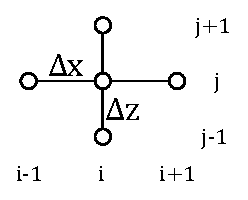
\includegraphics[height=5cm]{figures/pattern.eps}
    \caption{Шаблон на диференчната схема}
    \label{f:difference-pattern-1}
\end{figure}

Граничните условия \autoref{e:boundary-conditions-1} също искаме да апроксимираме с втори ред на точност. Знаем, че централна разлика от първи ред около възела има втори ред на точност в него. За да можем да я приложим, обаче, трябва да въведем фиктивни възли извън мрежата, както е показано на \autoref{f:finite-grid}. Това са черните възли, които не принадлежат на дефинираната мрежа. Флуидът не стига до тях, но въпреки това, можем да ги използваме, за да намерим стойностите на търсената мрежова функция по границата.

\begin{figure}[h]
    \centering
    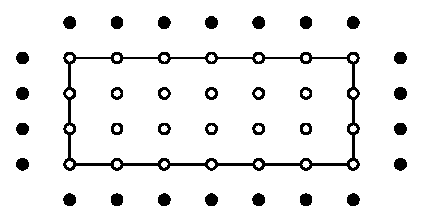
\includegraphics[height=5cm]{figures/difference-scheme.eps}
    \caption{Мрежа на дискретизацията}
    \label{f:finite-grid}
\end{figure}

Производните от граничните условия заместваме с централни разлики от първи ред както следва:
\begin{equation}
    \label{e:boundary-conditions-finite-scheme}
    \begin{aligned}
        &\left. \frac{\partial \Phi}{\partial x} \right|_{x=0}
        &&\rightarrow\quad
        \frac{y^n_{1,j} - y^n_{-1,j}}{2\Delta x} \\
        &\left. \frac{\partial \Phi}{\partial x} \right|_{x=L}
        &&\rightarrow\quad
        \frac{y^n_{N+1,j} - y^n_{N-1,j}}{2\Delta x} \\
        &\left. \frac{\partial \Phi}{\partial z} \right|_{z=-H}
        &&\rightarrow\quad
        \frac{y^n_{i,1} - y^n_{i,-1}}{2\Delta z}
    \end{aligned}
\end{equation}
В апроксимациите на граничните условия участват стойностите на решението във фиктивните възли. Ако построим линейна система с уравненията дотук, ще установим, че имаме повече неизвестни отколкото уравнения. Нека поискаме диференчното \autoref{e:main-equation-finite-diff} да бъде изпълнено и за възлите по границата. Тоест, прилагаме шаблона ,,кръст'' и в граничните възли. По този начин ще допълним системата с достатъчно уравнения.

Фиктивните възли искаме да изразим и премахнем от множеството неизвестни. Не е необходимо да пресмятаме стойността на търсената функция в тези точки. Напротив, това е дори в наша полза като по този начин работим с по-малка система. Но по-важно, запазваме структурата на системата.
\begin{equation}
    \label{e:boundary-conditions-finite-difference}
    \begin{aligned}
        \frac{y^n_{1,j} - y^n_{-1,j}}{2\Delta x} = 0 &\quad\Rightarrow\quad y^n_{-1,j} = y^n_{1,j} \\
        \frac{y^n_{N+1,j} - y^n_{N-1,j}}{2\Delta x} = 0 &\quad\Rightarrow\quad y^n_{N+1,j} = y^n_{N-1,j} \\
        \frac{y^n_{i,1} - y^n_{i,-1}}{2\Delta z} = 0 &\quad\Rightarrow\quad y^n_{i,-1} = y^n_{i,1}
    \end{aligned}
\end{equation}
Дотук диференчните апроксимации използват само възлите от един и същи времеви слой. Последните две гранични условия по свободната повърхност \autoref{e:kinematic-condition-linearized} и \autoref{e:dynamic-condition-linearized} включват производни и по времевата променлива. За тяхната дискретизация използваме схемата на ,,Кранк-Никълсън'', която апроксимира с втори ред на точност спрямо пространствената и времевата стъпка. Получената схема е от неявен вид и за всяка времева стъпка трябва да решим линейна алгебрична система с толкова неизвестни, колкото са възлите от мрежата $\omega$. Системата съставяме за неизвестните $\{y^{n+1}_{i,j}\}$, а стойностите на функцията на свободната повърхност изразяваме чрез полученото решение.

За динамичното гранично условие \autoref{e:dynamic-condition-linearized} имаме:
\begin{equation}
    \label{e:dynamic-condition-finite-difference}
    \left. \frac{\partial \Phi}{\partial t} \right|_{z=0} = -gh
    \quad\rightarrow\quad
    \frac{y^{n+1}_{i,M} - y^n_{i,M}}{\tau} = -\frac{g}{2} (h^{n+1}_i + h^n_i)
\end{equation}
От него можем да изразим в явен вид отместването на свободната повърхност в следващ момент $n+1$, ако вече сме намерили стойностите на потенциала за същия момент:
\begin{equation}
    \label{e:free-surface-finite-difference-formula}
    h^{n+1}_i = - \left[ h^n_i + \frac{2}{g} \frac{y^{n+1}_{i,M} - y^n_{i,M}}{\tau} \right]
\end{equation}
За кинематичното условие \autoref{e:kinematic-condition-linearized} правим дискретизацията:
\begin{equation}
    \label{e:kinematic-condition-finite-difference}
    \frac{\partial h}{\partial t} = \left. \frac{\partial \Phi}{\partial z} \right|_{z=0}
    \quad\rightarrow\quad
    \frac{h^{n+1}_i - h^n_i}{\tau}
    = \frac{1}{2} \left[ \frac{y^{n+1}_{i,M+1} - y^{n+1}_{i,M-1}}{2\Delta z} + \frac{y^n_{i,M+1} - y^n_{i,M-1}}{2\Delta z} \right]
\end{equation}
Нека изключим неизвестните стойности във фиктивните възли. От \autoref{e:main-equation-finite-diff}, приложено във възел $(i,M)$, изразяваме $y^n_{i,M+1}$:
\begin{equation}
    y^n_{i,M+1} = 2y^n_{i,M} - y^n_{i,M-1} - \frac{\Delta z^2}{\Delta x^2} (y^n_{i-1,M} - 2y^n_{i,M} + y^n_{i+1,M})
\end{equation}
Първо, преобразуваме лявата страна на дискретизацията от \autoref{e:kinematic-condition-finite-difference} като заместим \autoref{e:free-surface-finite-difference-formula}:
\begin{equation}
    \begin{aligned}
        \frac{h^{n+1}_i - h^n_i}{\tau}
        &= \frac{1}{\tau} \left[ - \left( h^n_i + \frac{2}{g} \frac{y^{n+1}_{i,M} - y^n_{i,M}}{\tau} \right) -h^n_i \right] \\
        &= -\frac{2}{\tau}h^n_i - \frac{2}{\tau^2 g}(y^{n+1}_{i,M} - y^n_{i,M})
    \end{aligned}
\end{equation}
След това нека разпишем дясната страна на \autoref{e:kinematic-condition-finite-difference}. Двете събираеми в дясната страна се различават само по времевия индекс. Достатъчно е да разпишем само едно от тях, а другото е аналогично:
\begin{equation}
    \begin{aligned}
        \frac{y^n_{i,M+1} - y^n_{i,M-1}}{2\Delta z}
        &= \frac{\left[ 2y^n_{i,M} - y^n_{i,M-1} - \frac{\Delta z^2}{\Delta x^2} (y^n_{i-1,M} - 2y^n_{i,M} + y^n_{i+1,M}) \right] - y^n_{i,M-1}}{2\Delta z} \\
        &= \frac{y^n_{i,M} - y^n_{i,M-1}}{\Delta z} - \frac{\Delta z}{2 \Delta x^2}(y^n_{i-1,M} - 2y^n_{i,M} + y^n_{i+1,M})
    \end{aligned}
\end{equation}
Така за реда възли от мрежата по свободната повърхност получихме:
\begin{equation}
    \label{e:top-row-finite-difference}
    \begin{aligned}
        - \frac{2}{\tau^2 g}(y^{n+1}_{i,M} - y^n_{i,M})
        = \frac{2}{\tau}h^n_i
        + \frac{1}{2} \left[ \vphantom{\frac{y^n_i}{\Delta z}} \right. &\frac{y^{n+1}_{i,M} - y^{n+1}_{i,M-1}}{\Delta z} - \frac{\Delta z}{2 \Delta x^2}(y^{n+1}_{i-1,M} - 2y^{n+1}_{i,M} + y^{n+1}_{i+1,M}) \\
        + & \left. \frac{y^n_{i,M} - y^n_{i,M-1}}{\Delta z} - \frac{\Delta z}{2 \Delta x^2}(y^n_{i-1,M} - 2y^n_{i,M} + y^n_{i+1,M}) \right]
    \end{aligned}
\end{equation}

\subsection{Съставяне на системата уравнения}
Нека съставим системата линейни алгебрични уравнения за неизвестните $\{y^{n+1}_{i,j}\}$. Можем да я запишем в матричен вид като $Ax=b$, където елементите на матрицата $A$ са коефициентите пред неизвестните стойности от $n+1$-ви слой, а във вектора $b$ участват всички членове от $n$-ти слой. Неизвестните $\{y^{n+1}_{i,j}\}$ номерираме с единствен индекс $p=j + iM$, тоест последователно по колони, за да получим новия вектор от неизвестни $\{x_p\}$. Избираме номерацията по колони, защото това ще доведе до по-малко изчисления в последствие.

С цел да избегнем потенциални грешки от закръгляния, заради крайната точност на представянето на числата в компютъра, при пресмятането на решението ще ,,нормализираме'' уравненията така, че елементите по диагонала да бъдат от един и същи порядък.

Във всички възли освен последния ред $j=M$ ползваме дискретизацията от \autoref{e:main-equation-finite-diff}, умножена с $\Delta x \Delta z$:
\begin{equation}
    - 2 \left( \frac{\Delta z}{\Delta x} + \frac{\Delta x}{\Delta z} \right) y^{n+1}_{i,j}
    + \frac{\Delta z}{\Delta x} (y^{n+1}_{i-1,j} + y^{n+1}_{i+1,j})
    + \frac{\Delta x}{\Delta z} (y^{n+1}_{i,j-1} + y^{n+1}_{i,j+1})
    = 0
\end{equation}
За възлите по трите непроницаеми граници ще ползваме същото уравнение като единствено заместим стойността на фиктивните възли използвайки \autoref{e:boundary-conditions-finite-difference}.

За реда $j=M$ използваме \autoref{e:top-row-finite-difference} с множител $2 \tau^2 g$. Прехвърляме всички членове от слоя $n+1$ към лявата страна и всички членове от слоя $n$ към дясната страна. Коефициентите пред членовете от лявата образуват матрицата $A$, а целият израз в дясно влиза във вектора $b$:
\begin{equation}
    \label{e:top-row-finite-difference-normalized}
    \begin{split}
        -\left( 4 + \frac{\tau^2 g}{\Delta z} + \frac{\tau^2 g \Delta z}{\Delta x^2} \right) y^{n+1}_{i,M}
        + \frac{\tau^2 g}{\Delta z} y^{n+1}_{i,M-1}
        + \frac{\tau^2 g \Delta z}{\Delta x^2} (y^{n+1}_{i-1,M} + y^{n+1}_{i+1,M}) \\
        = 4\tau g h^n_i
        - 4 y^n_{i,M}
        + \frac{\tau^2 g}{\Delta z} (y^n_{i,M} - y^n_{i,M-1})
        - \frac{\tau^2 g \Delta z}{2 \Delta x^2} (y^n_{i-1,M} - 2y^n_{i,M} + y^n_{i+1,M})
    \end{split}
\end{equation}
Отново за възлите в двата края ползваме \autoref{e:boundary-conditions-finite-difference}, за да премахнем стойностите във фиктивните възли.

\subsection{Решаване на системата уравнения}
Изборът на номерация определя кои от елементите на матрицата $A$ са ненулеви. Понеже шаблонът на диференчната схема е 5-точков, всеки ред от матрицта има най-много 5 ненулеви елемента. Тя е значително рядка. Тъй като имаме правоъгълна мрежа, ако изберем последователни индекси за съседните възли, ще получим диагонално-лентова матрица с размер на лентата $N+1$, ако номерираме по редове, или $M+1$, ако номерираме по колони. Размерите на басейна са такива, че при приблизително еднакъв размер на пространствените стъпки, ще получим по-малко възли в колона, отколкото в ред. Затова избрахме да номерираме по колони. Това означава, че размерът на лентата е по-малък и ще са необходими по-малко изчисления за намиране на решение.

Нещо повече, можем да видим, че при така номерирани възлите, матрицата е също и блоково три-диагонална. Можем да запишем системата в блоково-матричен вид както следва:
\medskip
\begin{equation}
    \label{f:block-tridiagonal}
    \left[
    \begin{array}{cccccc}
        C_0 & B_0    &         &         & \\
        A_1 & C_1    & B_1     &         & \\
            & \ddots & \ddots  & \ddots  & \\
            &        & A_{N-1} & C_{N-1} & B_{N-1} \\
            &        &         & A_N     & C_N
    \end{array}
    \right]
    \left[
    \begin{array}{c}
        X_0 \\ X_1 \\ \vdots \\ X_{N-1} \\ X_N
    \end{array}
    \right]
    = \left[
    \begin{array}{c}
        D_0 \\ D_1 \\ \vdots \\ D_{N-1} \\ D_N
    \end{array}
    \right]
\end{equation}
\medskip
където $\{A_j\}$, $\{B_j\}$ и $\{C_j\}$ са матрици с размери $(M+1)\times(M+1)$, а $\{X_j\}$ и $\{D_j\}$
са вектори с размери $M+1$. Матриците $\{C_j\}$ са също три-диагонални, защото всеки вътрешен възел има два съседни с последователни индекси. Другите два съседа са с индекси точно M+1 повече и по-малко. Те допринасят за матриците $\{A_j\}$ и $\{B_j\}$, които имат елементи само по диагонала.

Структурата на матрицата ни позволява лесно да я представим икономично като пазим в паметта единствено ненулевите елементи. За целта са ни необходими 5 вектора за всеки от ненулевите ленти. Така необходимата памет е от порядък $\mathcal{O}(N M)$, вместо $\mathcal{O}(N^2 M^2)$. Това подобрение е изключително важно за решаването на задачата с по-ситни мрежи и съответно повече възли и неизвестни.

Методите за решаване на линейни системи са разделени в два основни класа - директни и итерационни. Итерационните методи са по-прости от директните. Те започват от някакво начално приближение, което на всяка стъпка или итерация го подобряват. Основният им недостатък е, че може да са необходими голям брой итерации, за да постигнат желаната точност на решението. Някои итерационни методи са методът на Нютон и методът на релаксацията, чийто частен случай е методът на Зайдел\cite{linear-system-iterative-methods}.

Всеки итерационнен метод има нужда от критерий за спиране на итерациите. Най-често използваните са достигане на достатъчно малък резидуал $r^n=b-Ax^n$ или достатъчно малка разлика в решението между две съседни итерации.

\subsubsection{Метод на Зайдел}
Имаме зададено начално условие за потенциала, което ползваме като начално приближение за първата стъпка във времето. За всяка следваща стъпка ползваме полученото решение от предишната стъпка като начално приближение.

При метода на Зайдел, за да преминем от текущата стъпка към следващата, обновяваме последователно всеки елемент от вектора на текущото приближение използвайки формулите, съставящи матричното уравнение, като всеки път използваме обновените стойности на приближението.

Това можем да запишем формално като представим матрицата $A$ като сума от две триъгълни матрици:
\begin{equation}
    A = L + U
\end{equation}
където $L$ е долно-триъгълна матрица, включваща и диагонала на $A$, а $U$ е горно-триъгълна матрица. Системата придобива вида:
\begin{equation}
    Lx = b - Ux
\end{equation}
От където и определяме схемата за итериране:
\begin{equation}
    Lx^{n+1} = b - Ux^n
\end{equation}
Нека отбележим, че при различно, но отново последователно, номериране на възлите в мрежата ще получим схема за итериране, кояти има същия запис. На практика не използваме матричното равенство за итерациите, а изходните уравнения. Реда на обхождане на възлите все пак има влияние за сходимостта. При всяко обновяване на елемент се ,,предава'' информация за решението от следващата стъпка към обновения възел от неговите съседи. Затова бихме искали първо да обновим възли, чиито уравнения включват най-големи приноси от членове различни от съседните възли.

В \autoref{t:seidel-order-compare} са сравнени броя итерации, необходими за достигането на резидуал с $L_2$ норма по-малка от $10^{-6}$, между две имплементации на метода на Зайдел. При едната обхождаме възлите от дъното нагоре, а при другата - от свободната повърхност надолу. Стъпката по времето $\tau=0.005$ е достатъчно малка, за да не ограничава порядъка на точност.

\begin{table}[h]
    \centering
    \begin{tabular}{c|cccc}
        \toprule[1.5pt]
        Брой възли    & $10\times 3=30$ & $20\times 6=120$ & $40\times 12=480$ & $80\times 24=1920$ \\
        \midrule
        Обх. нагоре & 48              & 150              & 466 & 1362 \\
        Обх. надолу & 44              & 140              & 436 & 1272 \\
        \bottomrule[1.5pt]
    \end{tabular}
    \caption{Брой итерации при метода на Зайдел, в зависимост от реда на обхождане}
    \label{t:seidel-order-compare}
\end{table}

Наблюдаваме нужда от по-малък брой итерации в случая, когато започнем обновяването от възлите от свободната повърхност. Точно това бихме и очаквали, понеже тези възли единствено свързват стойностите от предходната стъпка с тези от текущата, и само те имат принос от отместването на свободната повърхност.

Друга характеристика на итерационните методи е, че те схождат по-бързо, когато матрицата има по-тежък диагонал. От \autoref{e:top-row-finite-difference-normalized} виждаме, че намалявайки стъпката по времето, диагоналът в последните $M+1$ реда ще стане относително по-голям от останалите елементи в редовете. Другите редове нямат зависимост от $\tau$, но все пак можем да видим разлика в броя итерации, необходими за достигането на резидуал със същата норма $10^{-6}$. В \autoref{t:seidel-step-size} са показани резултатите от експериментите с намаляване на стъпката по времето. Използвано е обхождането $j=M \dots 1$.

\begin{table}[h]
    \centering
    \begin{tabular}{c|cccc}
        \toprule[1.5pt]
        $\tau$            & $0.1$ & $0.05$ & $0.025$ & $0.0125$ \\
        \midrule
        $10\times 3=30$   & 70    & 58     & 52      & 46 \\
        $20\times 6=120$  & 214   & 184    & 164     & 150 \\
        $40\times 12=480$ & 726   & 644    & 578     & 516 \\
        \bottomrule[1.5pt]
    \end{tabular}
    \caption{Брой итерации при метода на Зайдел, в зависимост от размера на стъпката}
    \label{t:seidel-step-size}
\end{table}

Въпреки, че броя итерации е по-малък за по-малка стъпка, броя стъпки се увеличава по-бързо, отколкото броя итерации намалява. Изводът от експериментите е, че е най-добре да се избере максимален размер на стъпката, при която се достига желания порядък точност.

От \autoref{t:seidel-order-compare} можем да заключим, че броя итерации за една стъпка нараства приблизително линейно с броя възли в мрежата. На всяка итерация се правят $\mathcal{O}(NM)$ операции за обновяване на текущото приближение, което води до $\mathcal{O}(N^2 M^2)$ общ брой операции на стъпка.

Относно необходимата памет за този метод, той е оптимален, защото е нужно да пазим само ненулевите елементи от матрицата, и без никакви други допълнителни стойности. Тоест имаме $\mathcal{O}(NM)$ числа за матрицата и също толкова за дясната страна и за търсеното решение.

\subsubsection{Метод на матричната прогонка}
Директните методи за решаване на система линейни уравнения не ползват приближения както итерационните методи. При тях решението се смята чрез явни формули, като недостатъците са, че това може да бъде изключително бавно, и че преди края на пресмятането нямаме никакъв резултат. Някои директни методи са Гаусова елиминация, LU декомпозиция, метод на Холецки, метод на прогонката и др. Различните методи ползват различни характеристики на системата и е важно е да се избере този, който подхожда най-добре на задачата.

За нашата задача един вариант е метода за решаването на система с лентово-диагонална матрица. Той ползва $\mathcal{O}(np^2)$ операции\cite{band-matrix}, където $n=NM$ е броя неизвестни, а $p=M$ е дължината на лентата. Това дава порядък от $\mathcal{O}(NM^3)$ операции, което е сравнимо с метода на Зайдел, но малко по-добро, понеже $M<N$.

Вместо това, нека ползваме метода на прогонката, но записан за блоковете от матричното \autoref{f:block-tridiagonal}. Той се извежда, следвайки стъпките от Гаусовата елиминация. От първото блоково уравнение имаме:
\begin{equation}
    C_0 X_0 + B_0 X_1 = D_0
    \quad\Rightarrow\quad
    X_0 = \DefineAs{C_0^{-1}D_0}{F_0} - \DefineAs{C_0^{-1}B_0}{K_0} X_1
\end{equation}
Заместваме в следващото уравнение:
\begin{equation}
    \begin{aligned}
        A_1(F_0 &- K_0 X_1) + C_1 X_1 + B_1 X_2 = D_1 \\
        &\Rightarrow\quad \DefineAs{(C_1 - A_1 K_0)}{W_1}X_1 + B_1 X_2 = D_1 - A_1 F_0 \\
        &\Rightarrow\quad X_1 = \DefineAs{W_1^{-1}(D_1 - A_1 F_0)}{F_1} - \DefineAs{W_1^{-1}B_1}{K_1} X_2
    \end{aligned}
\end{equation}
Заместваме последователно в останалите уравнения по същия начин:
\begin{equation}
    \label{e:tridiag-recurrent}
    X_i = \DefineAs{W_i^{-1}(D_i - A_i F_{i-1})}{F_i} - \DefineAs{W_i^{-1}B_i}{K_i} X_{i+1}, \quad i=1\dots N-1
\end{equation}
Стигаме до последното уравнение, където намираме стойността на последния блок неизвестни:
\begin{equation}
    \begin{aligned}
        A_N(F_{N-1} &- K_{N-1}X_N) + C_N X_N = D_N \\
        &\Rightarrow\quad \DefineAs{(C_N - A_N K_{N-1})}{W_N}X_N = D_N - A_N F_{N-1} \\
        &\Rightarrow\quad X_N = \DefineAs{W_N^{-1}(D_N - A_N F_{N-1})}{F_N}
    \end{aligned}
\end{equation}
Сега остава само да се върнем назад в \autoref{e:tridiag-recurrent} и да намерим останалите неизвестни. Целият алгоритъм изглежда така:

\begin{enumerate}
    \item Дефинираме:
        \begin{align*}
            W_0 &= C_0, & W_i &= C_i - A_i K_{i-1}, &&i=1\dots N \\
            F_0 &= W_0^{-1} D_0, & F_i &= W_i^{-1}(D_i - A_i F_{i-1}), &&i=1\dots N \\
            K_0 &= W_0^{-1} B_0, & K_i &= W_i^{-1} B_i, &&i=1\dots N-1
        \end{align*}
    \item Намираме неизвестните по формулите:
        \begin{align*}
            X_N &= F_N \\
            X_i &= F_i - K_i X_{i+1}, \quad i=N-1 \dots 0
        \end{align*}
\end{enumerate}

Откъм брой операции, този метод също има порядък $\mathcal{O}(N M^3)$. Най-тежкото изчисление е намирането на обратните матрици $W_i^{-1}$. Те са $N+1$, като необходимите операции за една от тях са $\mathcal{O}(M^3)$. Умножения на матрици $W_i^{-1}B_i = K_i$ използва същия порядък операции.

Изискванията относно памет са по-високи от метода на Зайдел. Трябва да пазим всичките $N+1$ елементи от алгоритъма. Матриците $C_i$ са три-диагонални, но необходимите обратни матрици $W_i^{-1}$ са плътни. Паметта за тях е водеща и е от порядъка на $\mathcal{O}(N M^2)$.

\subsection{Локална грешка на апроксимацията}
Локалната грешка на апроксимацията се дефинира като разликата между лявата и дясната страна на апроксимиращото уравнение, пресметнати за точното решение. За да има съставената схема втори ред на точност, трябва локалната грешка на апроксимацията на диференциалното уравнение и на граничните условия да бъдат от порядъка на $\mathcal{O}(\Delta x^2 + \Delta z^2 + \tau^2)$. Началните условия са зададени точно и при тях нямаме грешка от апроксимация.

За локалната грешка на уравнението на Поасон имаме:
\begin{equation}
    \begin{aligned}
        \psi^n_{i,j} \, &
        \begin{aligned}
            = \frac{\partial^2 u^n_{i,j}}{\partial x^2} + \frac{\partial^2 u^n_{i,j}}{\partial z^2}
            - \left( \frac{u^n_{i-1,j} - 2u^n_{i,j} + u^n_{i+1,j}}{\Delta x^2} + \frac{u^n_{i,j-1} - 2u^n_{i,j} + u^n_{i,j+1}}{\Delta z^2} \right)
        \end{aligned}
        \\
        &
        \begin{aligned}
            = \frac{\partial^2 u^n_{i,j}}{\partial x^2} + \frac{\partial^2 u^n_{i,j}}{\partial z^2}
        \end{aligned}
        \\
        &
        \hspace{4em}
        \begin{aligned}
            - \frac{1}{\Delta x^2} \left( \vphantom{\frac{\partial u^n_{i,j}}{\partial x}} \right. &\cancel{u^n_{i,j}} - \cancel{\Delta x \frac{\partial u^n_{i,j}}{\partial x}} + \frac{\Delta x^2}{2} \frac{\partial^2 u^n_{i,j}}{\partial x^2} - \cancel{\frac{\Delta x^3}{6}\frac{\partial^3 u^n_{i,j}}{\partial x^3}} -\cancel{2u^n_{i,j}} \\
            + &\cancel{u^n_{i,j}} + \cancel{\Delta x \frac{\partial u^n_{i,j}}{\partial x}} + \frac{\Delta x^2}{2} \frac{\partial^2 u^n_{i,j}}{\partial x^2} + \cancel{\frac{\Delta x^3}{6}\frac{\partial^3 u^n_{i,j}}{\partial x^3}} \left. \vphantom{\frac{\partial u^n_{i,j}}{\partial x}} + \mathcal{O}(\Delta x^4) \right)
        \end{aligned}
        \\
        &
        \hspace{4em}
        \begin{aligned}
            - \frac{1}{\Delta z^2} \left( \vphantom{\frac{\partial u^n_{i,j}}{\partial x}} \right. &\cancel{u^n_{i,j}} - \cancel{\Delta z \frac{\partial u^n_{i,j}}{\partial z}} + \frac{\Delta z^2}{2} \frac{\partial^2 u^n_{i,j}}{\partial z^2} - \cancel{\frac{\Delta z^3}{6}\frac{\partial^3 u^n_{i,j}}{\partial z^3}} -\cancel{2u^n_{i,j}} \\
            + &\cancel{u^n_{i,j}} + \cancel{\Delta z \frac{\partial u^n_{i,j}}{\partial z}} + \frac{\Delta z^2}{2} \frac{\partial^2 u^n_{i,j}}{\partial z^2} + \cancel{\frac{\Delta z^3}{6}\frac{\partial^3 u^n_{i,j}}{\partial z^3}} \left. \vphantom{\frac{\partial u^n_{i,j}}{\partial x}} + \mathcal{O}(\Delta z^4) \right)
        \end{aligned}
        \\
        &
        \begin{aligned}
            = \frac{\partial^2 u^n_{i,j}}{\partial x^2} + \frac{\partial^2 u^n_{i,j}}{\partial z^2}
            - \frac{\partial^2 u^n_{i,j}}{\partial x^2} - \frac{\partial^2 u^n_{i,j}}{\partial z^2}
            + \mathcal{O}(\Delta x^2 + \Delta z^2)
        \end{aligned}
        \\
        &
        \begin{aligned}
            = \mathcal{O}(\Delta x^2 + \Delta z^2)
        \end{aligned}
    \end{aligned}
\end{equation}
За граничните условия имаме по две уравнения - едно от апроксимацията на самото условие и още едно от прилагането на шаблона ,,кръст''. За алгебричната система ползвахме второто, като изключихме стойността във фиктивния възел чрез първото. В системата можем да включим което и да е от двете, но само първото апроксимира граничното условие с търсения ред.

Ще покажем само за лявата граници, а останалите са аналогични. Ползваме шаблона ,,кръст'', за да изразим стойността във фиктивния възел:
\begin{equation}
    \begin{aligned}
        \frac{y^n_{-1,j} - 2y^n_{0,j} + y^n_{1,j}}{\Delta x^2} + &\frac{y^n_{0,j-1} - 2y^n_{0,j} + y^n_{0,j+1}}{\Delta z^2} = 0\\
        &\Rightarrow\quad
        y^n_{-1,j} = 2y^n_{0,j} - y^n_{1,j} - \frac{\Delta x^2}{\Delta z^2}(y^n_{0,j-1} - 2y^n_{0,j} + y^n_{0,j+1})
    \end{aligned}
\end{equation}
Така граничното условие се апроксимира чрез:
\begin{equation}
    \begin{aligned}
        \frac{y^n_{1,j} - y^n_{-1,j}}{2 \Delta x}
        &= \frac{y^n_{1,j} - 2y^n_{0,j} + y^n_{1,j}}{2 \Delta x} + \frac{1}{2\Delta x}\frac{\Delta x^2}{\Delta z^2}(y^n_{0,j-1} - 2y^n_{0,j} + y^n_{0,j+1}) \\
        &= \frac{y^n_{1,j} - y^n_{0,j}}{\Delta x} + \frac{\Delta x}{2\Delta z^2}(y^n_{0,j-1} - 2y^n_{0,j} + y^n_{0,j+1})
    \end{aligned}
\end{equation}
Тогава локалната грешка на апроксимация е:
\begin{equation}
    \label{e:local-error-boundary-condition}
    \begin{aligned}
        \psi^n_{0,j} \, &
        \begin{aligned}
            = \frac{\partial u^n_{0,j}}{\partial x} - \left( \frac{u^n_{1,j} - u^n_{0,j}}{\Delta x} + \frac{\Delta x}{2\Delta z^2}(u^n_{0,j-1} - 2u^n_{0,j} + u^n_{0,j+1}) \right)
        \end{aligned}
        \\
        &
        \begin{aligned}
            = \frac{\partial u^n_{0,j}}{\partial x} - \frac{1}{\Delta x} \left( \cancel{u^n_{0,j}} + \Delta x \frac{\partial u^n_{0,j}}{\partial x} + \frac{\Delta x^2}{2}\frac{\partial^2 u^n_{0,j}}{\partial x^2} + \mathcal{O}(\Delta x^3) - \cancel{u^n_{0,j}} \right)
        \end{aligned}
        \\
        &
        \hspace{4em}
        \begin{aligned}
            - \frac{\Delta x}{2 \Delta z^2} \left(\vphantom{\frac{\partial u^n_{0,j}}{\partial z}}\right. & \cancel{u^n_{0,j}} - \cancel{\Delta z \frac{\partial u^n_{0,j}}{\partial z}} + \frac{\Delta z^2}{2}\frac{\partial^2 u^n_{0,j}}{\partial z^2} - \cancel{\frac{\Delta z^3}{6}\frac{\partial^3 u^n_{0,j}}{\partial z^3}} - \cancel{2 u^n_{0,j}} \\
            + & \cancel{u^n_{0,j}} + \cancel{\Delta z \frac{\partial u^n_{0,j}}{\partial z}} + \frac{\Delta z^2}{2}\frac{\partial^2 u^n_{0,j}}{\partial z^2} + \cancel{\frac{\Delta z^3}{6}\frac{\partial^3 u^n_{0,j}}{\partial z^3}} + \mathcal{O}(\Delta z^4) \left. \vphantom{\frac{\partial u^n_{0,j}}{\partial z}} \right)
        \end{aligned}
        \\
        &
        \begin{aligned}
            = \frac{\partial u^n_{0,j}}{\partial x} - \frac{\partial u^n_{0,j}}{\partial x} - \frac{\Delta x}{2} \cancelto{0}{\left( \frac{\partial^2 u^n_{0,j}}{\partial x^2} + \frac{\partial^2 u^n_{0,j}}{\partial z^2} \right)}
            + \mathcal{O}(\Delta x^2) + \mathcal{O}(\Delta x \Delta z^2)
        \end{aligned}
        \\
        &
        \begin{aligned}
            = \mathcal{O}(\Delta x^2 + \Delta x\Delta z^2)
        \end{aligned}
    \end{aligned}
\end{equation}
Апроксимациите на граничните условия \autoref{e:dynamic-condition-finite-difference} и \autoref{e:kinematic-condition-finite-difference} при свободната повърхност развиваме в ред на Тейлър около момента $t = (n+\frac{1}{2})\tau$. Спрямо него следната апроксимацията:
\begin{equation}
    \label{e:local-error-time-deriv}
    \begin{aligned}
        \frac{u^{n+1} - u^n}{\tau} &=
        \frac{1}{\tau} \left( \cancel{u^{n+\frac{1}{2}}} + \frac{\tau}{2}\frac{\partial u^{n+\frac{1}{2}}}{\partial t} + \cancel{\frac{\tau^2}{8}\frac{\partial^2 u^{n+\frac{1}{2}}}{\partial t^2}} + \mathcal{O}(\tau^3) \right) \\
        &- \frac{1}{\tau} \left( \cancel{u^{n+\frac{1}{2}}} - \frac{\tau}{2}\frac{\partial u^{n+\frac{1}{2}}}{\partial t} + \cancel{\frac{\tau^2}{8}\frac{\partial^2 u^{n+\frac{1}{2}}}{\partial t^2}} + \mathcal{O}(\tau^3) \right) \\
        &= \frac{\partial u^{n+\frac{1}{2}}}{\partial t} + \mathcal{O}(\tau^2)
    \end{aligned}
\end{equation}
има втори ред на точност. Може също да се разглежда като централна разлика с половин стъпка.

За динамичното условие \autoref{e:dynamic-condition-finite-difference} имаме:
\begin{equation}
    \psi^{n+\frac{1}{2}}_{i,M} = \left( \frac{\partial u^{n+\frac{1}{2}}_{i,M}}{\partial t} - \frac{u^{n+1}_{i,M} - u^n_{i,M}}{\tau} \right) + g\left( h^{n+\frac{1}{2}}_i - \frac{h^{n+1}_i + h^n_i}{2} \right)
\end{equation}
Първият член е идентичен с \autoref{e:local-error-time-deriv}. За втория член правим подобен извод:
\begin{equation}
    \begin{aligned}
        \frac{h^{n+1}_i + h^n_i}{2} &= \frac{1}{2} \left( h^{n+\frac{1}{2}}_i + \cancel{\frac{\tau}{2}\frac{\partial h^{n+\frac{1}{2}}_i}{\partial t}} + \mathcal{O}(\tau^2)
        + h^{n+\frac{1}{2}}_i - \cancel{\frac{\tau}{2}\frac{\partial h^{n+\frac{1}{2}}_i}{\partial t}} + \mathcal{O}(\tau^2) \right) \\
        &= h^{n+\frac{1}{2}}_i + \mathcal{O}(\tau^2)
    \end{aligned}
\end{equation}
Използвайки изводите от \autoref{e:local-error-boundary-condition} и \autoref{e:local-error-time-deriv} получаваме същия резултат за кинематичното условие \autoref{e:kinematic-condition-finite-difference}:
\begin{equation}
    \begin{aligned}
        \psi^{n+\frac{1}{2}}_{i,M} \, &
        \begin{aligned}
            = \left( \frac{\partial h^{n+\frac{1}{2}}_i}{\partial t} - \frac{h^{n+1}_i - h^{n}_i}{\tau} \right)
        \end{aligned}
        \\
        &
        \hspace{4em}
        \begin{aligned}
            - \left( \frac{\partial u^{n+\frac{1}{2}}_{i,M}}{\partial z} - \frac{1}{2}\left(\frac{u^{n+1}_{i,M+1} - u^{n+1}_{i,M-1}}{2\Delta z} + \frac{u^{n}_{i,M+1} - u^{n}_{i,M-1}}{2\Delta z}\right)\right)
        \end{aligned}
        \\
        &
        \begin{aligned}
            = \mathcal{O}(\tau^2) - \left( \frac{\partial u^{n+\frac{1}{2}}_{i,M}}{\partial z} - \frac{1}{2}\left(\frac{\partial u^{n+1}_{i,M}}{\partial z} + \frac{\partial u^{n}_{i,M}}{\partial z} + \mathcal{O}(\Delta z^2 + \Delta z\Delta x^2)\right)\right)
        \end{aligned}
        \\
        &
        \begin{aligned}
            = \mathcal{O}(\tau^2) - \left( \frac{\partial u^{n+1}_{i,M}}{\partial z} - \frac{\partial u^{n+1}_{i,M}}{\partial z} + \mathcal{O}(\tau^2 + \Delta z^2 + \Delta z\Delta x^2)\right)
        \end{aligned}
        \\
        &
        \begin{aligned}
            = \mathcal{O}(\Delta x^2 + \Delta z^2 + \tau^2)
        \end{aligned}
    \end{aligned}
\end{equation}
С това показахме, че съставената схема има втори ред на точност. За да намерим практически този ред ползваме метода на Рунге. При него пресмятаме решението в няколко мрежи с двойно по-малки стъпки, така че точките от най-едрата мрежа да съвпадат с точки от всички по-ситни мрежи. Тоест, всички мрежи имат общи точки, в които ще пресметнем решението. Трябва да предположим, че грешката е пропорционална на константа $C$, която е приблизително еднаква за всички мрежи. Така грешката на решението $e_h$ за някой избор на стъпка $h = max(\Delta x, \Delta z, \tau)$ очакваме да бъде също пропорционална на $h^k$, където $k$ е търсения ред на точност. За фиксиран възел от мрежата:
\begin{equation}
    e_h = u_h - y_h = Ch^k
\end{equation}
Ако не знаем точното решение, то ни трябват приближенията от три последователни мрежи. Разглеждаме разликите:
\begin{equation}
    \begin{aligned}
        y_{\frac{h}{2}} - y_h
        &= \left( \cancel{u_{\frac{h}{2}}} - C\left(\frac{h}{2}\right)^k \right) - \left( \cancel{u_h} - Ch^k \right)
        = Ch^k \left( 1 - \frac{1}{2^k} \right) \\
        y_{\frac{h}{4}} - y_{\frac{h}{2}}
        &= \left( \cancel{u_{\frac{h}{4}}} - C\left(\frac{h}{4}\right)^k \right) - \left( \cancel{u_{\frac{h}{2}}} - C\left(\frac{h}{2}\right)^k \right)
        = C\left(\frac{h}{2}\right)^k \left( 1 - \frac{1}{2^k} \right)
    \end{aligned}
\end{equation}
Можем да съкратим члена от точното решение, понеже точките от двете мрежи съвпадат, а решението е едно и също. Тогава редът на точност извеждаме от израза:
\begin{equation}
    \frac{y_{\frac{h}{2}} - y_h}{y_{\frac{h}{4}} - y_{\frac{h}{2}}}
    = \frac{Ch^k\left( 1 - \frac{1}{2^k} \right)}{C\left(\frac{h}{2}\right)^k \left( 1 - \frac{1}{2^k} \right)}
    = 2^k
    \quad\Rightarrow\quad
    k = log_2\left\vert \frac{y_{\frac{h}{2}} - y_h}{y_{\frac{h}{4}} - y_{\frac{h}{2}}} \right\vert
\end{equation}
В нашия случай знаем точното решение и можем да намерим същия ред само с две приближения като:
\begin{equation}
    \frac{e_h}{e_{\frac{h}{2}}} = \frac{Ch^k}{C\frac{h^k}{2^k}} = 2^k
    \quad\Rightarrow\quad
    k = log_2\left\vert \frac{e_h}{e_{\frac{h}{2}}} \right\vert
\end{equation}
Преди да приложим тези формули в действие, има няколко детайла, които трябва да вземем впредвид. Грешката може да си сменя знака. Затова трябва да подсигурим положителност на аргумента на логаритъма.
Освен това, тази оценка е за всеки възел поотделно. За да включим всичките възли, съставяме вектор от грешките като ги преномерираме с един индекс, вместо три. Самата преномерация няма значение. Възлите в началния момент ги пропускаме, понеже тяхната стойност е определена от началното условие, което е еднакво за всички по-ситни мрежи. Тоест грешката не би се променила и практичния ред на сходимост е 0. Това би отклонило същинския резултат.

\begin{figure}[h]
    \centering
    \includegraphics{figures/results/convergence-rate.eps}
    \caption{Ред на точност на приближеното решение}
    \label{f:conv-rate}
\end{figure}

На \autoref{f:conv-rate} е показан редът на точност за потенциала на скоростите $\Phi(x,z,t)$ и отместването на свободната повърхност $h(x,t)$ в две различни векторни норми, в зависимост от броя надробявания на мрежата. Броят интервали за първата мрежа е $(6,3,6)$ съответно по $(x, z, t)$. Нормата прилагаме върху вектора от грешки, след което вземаме логаритъм. Виждаме, че оценката за реда на точност съвпада с този, получен аналитично. От графиката можем да направим извод, че както средната грешка, така и максималната грешка, спадат 4 пъти, когато стъпките на мрежата се смаляват 2 пъти.

От това, че прилагаме норма преди логаритъма, се губи информацията за реда на точност за индивидуален възел. Може би в някой възел грешката има различен характер. Друга възможност за съставяне на графиката е да вземем средния или минималния ред на точност от всички точки. \autoref{f:conv-rate-averaged} показва точно това. Виждаме, че евентуално грешките във всички възли спадат достатъчно бързо.

\begin{figure}[h]
    \centering
    \includegraphics{figures/results/convergence-rate-average.eps}
    \caption{Среден и минимален ред на точност от всички точки}
    \label{f:conv-rate-averaged}
\end{figure}

След като знаем и точното решение, можем да видим и истинската грешка на всяка една мрежа. Това е показано на \autoref{f:error-rate}, отново чрез две норми.

\begin{figure}[h]
    \centering
    \includegraphics{figures/results/error-rate.eps}
    \caption{Грешката на приближеното решение}
    \label{f:error-rate}
\end{figure}

Линейната тенденция на графиката в логаритмична скала подсказва, че грешката е пропорционална на стъпката с константна експонента.

\subsection{Резултати}
С цел да сравним полученото числено решение на задачата с точното решение, трябва едната функция да приведем в пространството на другата, понеже двете функции са в различни пространства. Едната възможност е непрекъснатата функция на точното решение да ограничим само в точките от възлите на мрежата, а другата - да интерполираме мрежовата функция, например с линейна интерполация по всяко измерение.

За валидация на числената схема нека сравним численото решение с аналитичното. Ще ползваме отново същите параметри на задачата както при \autoref{f:compare-linear-solution}. Вземаме разликите между стойностите от точното решение и намереното числено във възлите от мрежата, което ни дава истинската грешка. Тази грешка можем да интерполираме с вградената функция $Interpolation[]$ в програмния език Mathematica.

\begin{figure}[h]
    \centering
    \begin{subfigure}[b]{0.47\textwidth}
        \includegraphics[width=\textwidth]{figures/results/error-solution-h-0.005.eps}
        \caption{H=0.005}
    \end{subfigure}
    \hfill
    \begin{subfigure}[b]{0.47\textwidth}
        \includegraphics[width=\textwidth]{figures/results/error-solution-h-0.025.eps}
        \caption{H=0.025}
    \end{subfigure}
    \caption{Грешка между точното и численото решение}
    \label{f:compare-numeric-solution-linear}
\end{figure}

Използваната резолюция на мрежата за изобразеното числено решение във \autoref{f:compare-numeric-solution-linear} е $\Delta x=0.01, \Delta z = \tau = min(0.01, H)$. Показана е абсолютната грешка на функцията на свободната повърхност. Виждаме, че грешката расте с нарастване на времето $t$. Това е очаквано, понеже на всяка стъпка правим малка грешка, която се събира постепенно. Ако съдим по графиката на \autoref{f:error-accumulated-linear}, тя расте линейно. Виждат се и скокове в грешката, когато вълната срещне граница или премине другата си половина.

\begin{figure}[h]
    \centering
    \includegraphics{figures/results/error-accumulated.eps}
    \caption{Грешката на решението нараства с течение на времето}
    \label{f:error-accumulated-linear}
\end{figure}

\subsection{Добавяне на бутало към численото решение}
По-рано видяхме, че метода ,,разделяне на променливите'' не допуска съществуването на бутало, което се движи с равна скорост по цялата му дълбочина. Използвайки числено решение ще заобиколим това ограничение. Нека разгледаме отново функцията, описваща хоризонталното отместване на буталото спрямо дясната граница $P(t)$. Очевидно тя трябва да бъде непрекъсната, но изключвайки това сме свободни да я изберем.

Промяната на това гранично условие трябва да се отрази в диференчната схема. Хоризонталната скорост на флуида трябва да е равна на скоростта на буталото. За възлите от най-дясната колона променяме дясната страна от \autoref{e:boundary-conditions-finite-difference}:
\begin{equation}
    \frac{y^n_{N+1,j} - y^n_{N-1,j}}{2\Delta x} = P'(t_n) \quad\Rightarrow\quad y^n_{N+1,j} = y^n_{N-1,j} + 2\Delta x P'(t_n)
\end{equation}
Функцията $P(t)$ ни е известна, така че знаем и нейната производна $P'(t)$. Приносът към системата от алгебрични уравниния е само във вектора на дясната страна. Матрицата ѝ остава непроменена.

Добавянето на бутало ни дава нови възможностти да взаимодействаме с водната повърхност. Нека зададем конкретен режим на движение и видим какво ще се получи.

\subsubsection{Генериране на стоящи вълни}
Нека разгледаме басейн с нови размери. Избираме дължина $L=100$m и дълбочина от водната повърхност $H=2$m. Дискретизираме със стъпка $0.05$m по всяко измерение, с максимално време $t_{max}=80$s. Началното условие оставяме същото. За функцията на буталото избираме хармонично движение с период $8$s, което започва и завършва плавно, а след това спира. Скоростта е показано на \autoref{f:piston-vel-1}. Максималното отместване е $1.5$m.

\begin{figure}[h]
    \centering
    \includegraphics{figures/results/piston-vel-1.eps}
    \caption{Функция, описваща скоростта на дясната граница}
    \label{f:piston-vel-1}
\end{figure}

Бихме очаквали периодично движение да генерира еднакви по дължина вълни. Те ще се движат с еднаква скорост и ще стигнат до другата граница, където ще се отразят. Когато това стане, те ще срещнат вълните зад тях и от принципа за суперпозиция очакваме да получим стояща вълна. Численото решение е показано на \autoref{f:piston-solution}.

\begin{figure}[h]
    \centering
    \includegraphics{figures/results/piston-wave-1.eps}
    \caption{Вълни, образувани от движението на буталото}
    \label{f:piston-solution}
\end{figure}

От графиката се вижда, че вълните не променят формата си. Това отчасти се дължи на факта, че са генерирани от хармонично движение, но тяхната дължина е значително голяма сравнено с дълбочината на басейна. Това ги категоризика по-близо до плитки вълни, за които знаем, че са недисперсионни. Можем да намерим теоретичната скорост на тези вълни спрямо периода на движението. Периода на вълната е времето, за което фиксирана точка прави един пълен цикъл. За същото време фиксирана точка ще измине една дължина на вълната. Следователно имаме:
\begin{equation}
    T = \frac{\lambda}{c} = \frac{\lambda}{\sqrt{\frac{\lambda g}{2\pi}tanh(\frac{2\pi H}{\lambda})}}
\end{equation}
Използваме итеративен метод за намирането на корен на това уравнение. Спомняйки си, че $T=8$s, намираме $\lambda \approx 34.3$m. Това ни дава скоростта $c \approx 4.28$m/s. Ако проследим правите линии от графиката, които тресират фиксирани точки от вълната, виждаме, че всяка точка измината $100$m за $\approx 24$s, което ни дава емперична скорост от $4.17$m/s. Можем да направим заключението, че бутало, което се движи хармонично с фиксирана честота, образува вълни със същата честота. Тогава техните амплитуди можем да предположим, че зависят от максималното отместване на буталото.

\clearpage
\section{Заключение}
В дипломната работа са определени какво представляват вълните и са дадени примери за различни видове вълни. Представени са основните физични закони, от които са изведени уравненията на движение за произволен флуид. Описана е задачата, която стремим да решим. Направени са опростявания спрямо предположенията за флуида и спецификите на задачата, за да получим линеаризиран модел. За него е изведено аналитично решение със зададено начално условие. Съставена е диференчна схема за задачата по метода на крайните разлики. Предложени са два варианта за решаване на съставената линейна алгебрична система и са изследвани техните предимства и недостатъци. Валидирана е коректността на схемата както теоретично, така и експериментално със сравнения спрямо аналитичното решение.

\section{Бъдещо развитие}
Линейният модел е доста ограничен и не особено реалистичен за предсказването на точното поведение на вълните. Например, той позволява произволна амплитуда на вълната, а в реалния свят тя има максимална височина спрямо дължината ѝ, след която тя се разбива. Разглеждането на нелинейни модели би довело до по-естествено поведение. Нейната скорост зависи също от амплитуда ѝ, понеже разликата между най-ниската точка и най-високата е достатъчна голяма. Един конкретен нелинеен модел е този на Korteweg-De Vries, който позволява както периодични вълни, така и самостоятелни недесперсионни вълни, още познати като солитони. Той е единствено за двумерни задачи и разглежда само водната повърхност, но не и под нея.

Методът на крайните разлики се затруднява с неправилна геометрия на границите на задачата. За басейни с наклонени стени, дъно, или подводни препятствия е по-подходящо ползването на дискретизация, която може да се справи с нерегулярни форми. Такива методи са методът на крайните елементи или методът на крайните обеми.

Ако искаме да моделираме ефекта от разбиването на вълната е необходимо да можем да проследим къде е границата между водата и атмосферата. Съществуват множество техники, които позволяват това, някои от които са Marker-and-cell (MAC) схемата и техниката Smoothed-particle hydrodynamics (SPH).

Разглеждането на зависимостта между дължината на вълната и движението на бутало, което я генерира, може да послужи за по-дълбоко разбиране на движението на гравитационните вълни. С подобен модел би могло да се генерират точно избрани вълни, което е необходимо за физически експерименти.

\clearpage
\section{Приложение}
\appendix
% Using subsections as sections for the appendix to appear indented in the contents. Each appendix is its own subsection

% Change the equation numbering to use the subsection letter (e.g. A.1, A.2)
\numberwithin{equation}{subsection}

% Make the subsections for the appendix count with letters
\renewcommand{\thesubsection}{\Alph{subsection}}

\subsection{Формула на Лайбниц}
\label{a:leib-proof}
\begin{equation}
    \label{e:leib-main}
    \frac{d}{dt}\int_{V(t)}A(\mathbf{x}, t) dV = \int_{V(t)}\frac{dA}{dt}+A( \nabla\cdot\vec{u})  dA
\end{equation}
Формулата на Лайбниц ни казва как да диференцираме интеграл с подвижни граници. Ще докажем, че тя е валидна за скаларна и векторна функция $A$.

Разглеждаме обем $V(t)$ заграден от повърхност $S(t)$, която се изменя със скорост $\vec{u}(\mathbf{x}, t)$ (\autoref{f:leib-fig}). Нека:
\begin{equation}
    I(t):=\int_{V(t)}A(\mathbf{x}, t)dV
\end{equation}
където $A(\mathbf{x}, t)$ е непрекъсната функция с непрекъснати частни производни. За краткост дефинираме:
\begin{equation}
    \begin{aligned}
        A^\prime(\mathbf{x}, t)&:=A(\mathbf{x}, t+\Delta t) \\
        V^\prime(t)&:=V(t+\Delta t) \\
        S^\prime(t)&:=S(t+\Delta t)
    \end{aligned}
\end{equation}
От дефиницията на производна имаме:
\begin{equation}
    \label{e:leib-parts}
    \begin{aligned}
        \frac{dI}{dt}&=\underset{\Delta t \rightarrow 0}{\lim}\frac{1}{\Delta t} \left( \int_{V^\prime}A^\prime dV -\int_{V}AdV \right) \\
        &=\underset{\Delta t \rightarrow 0}{\lim}\frac{1}{\Delta t} \left(\left[ \int_{V^\prime}A^\prime dV -\int_{V}A^\prime dV \right] + \left[ \int_{V}A^\prime dV -\int_{V}AdV \right] \right) \\
        &=\underset{\Delta t \rightarrow 0}{\lim}\frac{1}{\Delta t} \left( \int_{V^\prime -V}A^\prime dV +\int_{V}A^\prime-A dV \right) \\
        &=\underset{\Delta t \rightarrow 0}{\lim}\frac{1}{\Delta t} \left( \int_{V^\prime -V}A^\prime dV \right) +\int_{V}\frac{\partial A}{\partial t} dV
    \end{aligned}
\end{equation}
В последното равенство първият член се получава от "събирането"\space на двата ориeнтирани обема, понеже подинтегралната функция е еднаква. Единият се добавя, а другият се изважда. В тяхното сечение ($V\cap V^\prime$) резултатът е 0.

\begin{figure}[h]
    \centering
    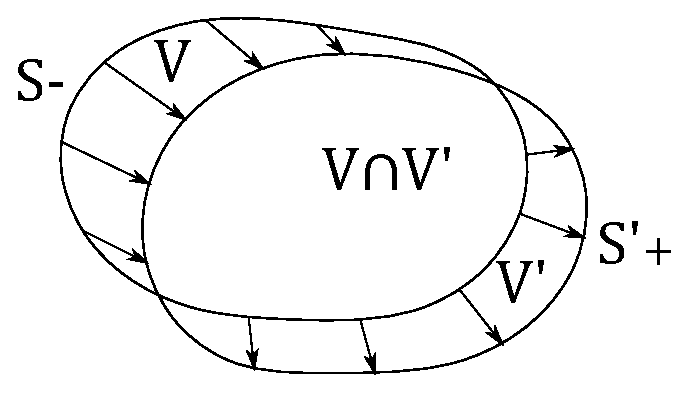
\includegraphics{figures/leib_proof.eps}
    \caption{Подвижен обем $V$ в два близки момента}
    \label{f:leib-fig}
\end{figure}

Нека разгледаме повърхността, заграждаща обединението на двата обема. Частта, принадлежаща на $V$, обозначаваме с $S-$, а тази принадлежаща на $V^\prime$ - с $S^\prime+$. Тогава можем да изразим интеграла от обем в двете области, невключващи сечението, чрез интеграл по повърхността:
\begin{equation}
    \int_{V^\prime -V}A^\prime dV=\int_{S^\prime+}A^\prime (\vec{u}\cdot\vec{n})\Delta t dS - \int_{S-}A^\prime (\vec{u}\cdot(-\vec{n}))\Delta t dS
\end{equation}
където $\vec{u}$ отново е скоростта на повърхността на обема, а $\vec{n}$ е външната нормала. Диференциален обем $dV$ е равен на обем $|\vec{u}\cdot\vec{n}|\Delta tdS$ на паралелипипед с основа $dS$, сключваща ъгъл с косинус $\vec{u}\cdot\vec{n}$ със височина, имаща дължина $\Delta t$. Функцията $A^\prime$ в тези обеми е равна на стойността и по повърхността с точност до линейни членове по пространствените променливи.

Сега можем да направим граничния преход:
\begin{equation}
    \label{e:leib-limit}
    \begin{aligned}
        \underset{\Delta t \rightarrow 0}{\lim}\frac{1}{\Delta t} \left( \int_{V^\prime -V}A^\prime dV \right) &= \underset{\Delta t \rightarrow 0}{\lim}\frac{1}{\cancel{\Delta t}} \left( \int_{S^\prime+}A^\prime (\vec{u}\cdot\vec{n})\cancel{\Delta t} dS - \int_{S-}A^\prime (\vec{u}\cdot(-\vec{n}))\cancel{\Delta t} dS \right) \\
        &= \underset{\Delta t \rightarrow 0}{\lim}\int_{(S-) \cup (S^\prime+)} A^\prime(\vec{u}\cdot\vec{n})dS \\
        &= \int_S A(\vec{u}\cdot\vec{n})dS
    \end{aligned}
\end{equation}
Прилагаме теоремата на Остроградски-Гаус за дивергенцията към последния резултат. В случая, когато $A$ е векторна функция, е необходимо да се ползва обобщената теорема за тензори\cite{div-theorem}:
\begin{equation}
    \int_V \frac{\partial A_{i_1,i_2,...,i_n}}{\partial x_{i_k}}dV=\int_{\partial V}A_{i_1,i_2,...,i_n}n_{i_k}dS
\end{equation}
За скаларна функция имаме:
\begin{equation}
    \begin{aligned}
        \int_S A(\vec{u}\cdot\vec{n})dS&=\int_V \nabla\cdot(A\vec{u}) dV \\
        &= \int_V A(\nabla\cdot\vec{u}) + \vec{u}\cdot(\nabla A) dV
    \end{aligned}
\end{equation}
За векторна функция резултатът ще е същия, но понеже тензорите и скаларното произведение с тях не комутират, трябва да се разпише по-внимателно:
\begin{equation}
    \label{e:div-apply}
    \begin{aligned}
        \int_S \vec{A}(\vec{u}\cdot\vec{n})dS&=\int_S A_i e_i u_j n_j dS \\
        &=\int_V \frac{\partial A_i u_j}{\partial x_j} e_i dV \\
        &=\int_V A_i e_i \frac{\partial u_j}{\partial x_j} + (u_j \frac{\partial}{\partial x_j}) A_i e_i dV \\
        &=\int_V \vec{A}(\nabla\cdot\vec{u}) + (\vec{u}\cdot\nabla) \vec{A} dV
    \end{aligned}
\end{equation}
Използваме резултатите от \autoref{e:div-apply} в \autoref{e:leib-limit} и от \autoref{e:leib-limit} в \autoref{e:leib-parts}, с което получаваме търсения резултат:
\begin{equation}
    \begin{aligned}
        \frac{d}{dt}\int_{V(t)}A dV &= \int_V \frac{\partial A}{\partial t} + A(\nabla\cdot\vec{u}) + (\vec{u}\cdot\nabla)A dV \\
        &= \int_V \frac{d A}{d t} + A(\nabla\cdot\vec{u}) dV
    \end{aligned}
\end{equation}
\subsection{Ортогонален базис от косинуси}
\label{a:cosin-basis}
Нека дефинираме скаларно произведение, без да доказваме, че наистина отговаря на условията за скаларно произведение:
\begin{equation}
    \label{e:cosine-scalar-prod}
    \langle f,g \rangle = \int_0^L fg dx
\end{equation}
Разглеждаме косинуси от вида $cos(k_n x) = cos(\frac{n \pi}{L} x)$. Искаме да покажем, че скаларното произведение между два косинуса с различен индекс е равно на нула:
\begin{equation}
    \label{e:cosine-orthogonal}
    \langle cos(k_n x),cos(k_m x) \rangle = 0, \quad n \neq m
\end{equation}
Ще приложим смяна на променливата в интеграла от \autoref{e:cosine-scalar-prod}:
\begin{align}
    x = \frac{L}{\pi} y && dx = \frac{L}{\pi}dy && y_0=0 && y_1=\cancel{L}\frac{\pi}{\cancel{L}}
\end{align}
Следователно:
\begin{equation}
    \begin{aligned}
        \int_0^L cos(\frac{n\pi}{L}x) \, cos(\frac{m\pi}{L}x) dx
        &= \frac{L}{\pi}\int_0^\pi cos(ny) \, cos(my) dy \\
        &= \frac{L}{\pi}\int_0^\pi \frac{cos((n-m)y) + cos((n+m)y)}{2} dy \\
        &= \frac{L}{2\pi}\left. \left( \frac{sin((n-m)y)}{n-m} + \frac{sin((n+m)y)}{n+m} \right) \right|_0^\pi \\
        &= 0
    \end{aligned}
\end{equation}
С това е доказано \autoref{e:cosine-orthogonal}. Нека също да видим какво се получава, когато вземем произведението между косинуси с еднакъв индекс:
\begin{equation}
    \begin{aligned}
        \int_0^L cos^2(\frac{n\pi}{L}x) dx
        &= \frac{L}{\pi}\int_0^\pi cos^2(ny) dy \\
        &= \frac{L}{n\pi}\int_0^\pi cos(ny) d \, sin(ny) \\
        &= \frac{L}{n\pi}\left( \left. \vphantom{\int} cos(ny)\cancelto{0}{sin(ny)} \quad \right|_0^\pi - \int_0^\pi sin(ny) d \, cos(ny) \right) \\
        &= \frac{L}{\cancel{n}\pi}\int_0^\pi \cancel{n} sin^2(ny) dy \\
        &= \frac{L}{\pi}\int_0^\pi 1 - cos^2(ny) dy \\
        &= \frac{L}{\pi} \left(\pi - \int_0^\pi cos^2(ny) dy \right) \\
        &= L - \int_0^L cos^2(\frac{n\pi}{L}x) dx
    \end{aligned}
\end{equation}
Така намерихме рекурентна връзка за скаларното произведение между косинуси с еднакъв индекс. Ако го означим с функция $f(n)$, можем да го изразим като:
\begin{equation}
    f(n) = L - f(n) \quad \Rightarrow \quad f(n) = \int_0^L cos^2(\frac{n\pi}{L}x) dx = \frac{L}{2}
\end{equation}
Тоест това скаларно произведение има една и съща стойност за произволно $n \neq 0$. В частния случай $n=0$ лесно се вижда, че стойността е $f(0)=L$.

\clearpage
\bibliographystyle{plain} % List in order of use
\bibliography{refs} % Entries are in the refs.bib file
\end{document}